\documentclass[letterpaper, 12pt]{article}

\usepackage{amssymb, amsthm, amsmath}
\usepackage[letterpaper, margin=1.25in]{geometry}
\usepackage{comment}
\usepackage{spverbatim}
\usepackage{tikz}
\usepackage{chngcntr}
\usepackage{indentfirst}
\usepackage{hyperref}
\usepackage{listings}
%\usepackage{appendix}

\title{Implementing Path Coloring Algorithms on Planar Graphs}
\author{Aven Bross}

\theoremstyle{definition}
\newtheorem{definition}{Definition}[section]

\theoremstyle{definition}
\newtheorem{example}{Example}[section]

\theoremstyle{thm}
\newtheorem{theorem}{Theorem}[section]

\theoremstyle{definition}
\newtheorem{algorithm}{Algorithm}[section]


\lstset{language=C++}


\pgfdeclarelayer{bg}    % declare background layer
\pgfsetlayers{bg,main}  % set the order of the layers

\tikzset{every picture/.append style={scale=1.1}}
\tikzset{every label/.append style={fill=white}}
\tikzset{
    every node/.style={circle, fill, draw, minimum size=1mm, scale=.6,
    	font=\LARGE}
}

\setcounter{secnumdepth}{1}
\counterwithin{figure}{section}

\begin{document}

\maketitle

\section*{Abstract}
A path coloring of a graph partitions its vertex set into color classes such
that each class induces a disjoint union of paths. In this project we consider
implementing several algorithms to compute path colorings of graphs embedded in
the plane.

We present two algorithms to path color plane graphs with $3$ colors
based on a proof by Poh's in 1990. First we describe a naive algorithm that
directly follows Poh's procedure, then we give a modified algorithm
that runs in linear time.

Independent results of Hartman and Skrekovski describe a procedure that takes
a plane graph $G$ and a list of $3$ colors for each vertex, and
computes a path coloring of $G$ such that each vertex receives a color from its
list. We present a linear time algorithm based on Hartman and Skrekovski's
proofs.

A C++ implementation is provided for all three algorithms, utilizing the Boost
Graph Library. Instructions are given on how to use the implementation
to construct colorings for plane graphs represented by Boost data
structures.

\section{Plane Graphs}

We will be concerned only with simple plane graphs. Informally, a plane graph
is a network drawn in the plane consisting of a set of points, and a set of
lines between points such that no lines cross.

Formally a \textit{simple graph} is an ordered pair $G=(V,E)$ consisting of a finite set
$V$ of \textit{vertices} and a set $E$ of two element subsets of $V$ known as
\textit{edges}. We will refer to the the vertex and edge sets of a graph $G$ by
$V(G)$ and $E(G)$, respectively. All graphs in this project are simple.

As shorthand we will denote an edge $\{u,v\}\in E(G)$ simply as $uv$ or $vu$.
Furthermore, if it is clear by context that $v\in V(G)$ is a vertex, or $uv\in
E(G)$ an edge, we will use the notation $v\in G$, or $uv,\in G$.

Two vertices $u,v\in V(G)$ are \textit{adjacent} if $uv\in E(G)$. Vertices $u$
and $v$ are known as the \textit{endpoints} of $uv$. The edge $uv$ is said to be
\textit{incident} to the vertices $u$ and $v$. The vertices in $G$ adjacent to a
vertex $v$ are known as the \textit{neighbors} of $v$. The number of neighbors
of a vertex $v$ is its \textit{degree}, denoted $\text{deg}(v)$.

A graph $H$ is a \textit{subgraph} of $G$ if $V(H)\subseteq V(G)$ and
$E(H)\subseteq E(G)$. If $S\subseteq V(G)$ the \textit{induced subgraph} of
$S$ on $G$ is the subgraph $H$ defined by $V(H)=S$ and
$E(H)=\{uv\in E(G) \ | \ u,v\in S\}$. We say a subgraph $H$ of a graph $G$ is
\textit{induced} if it is the induced subgraph of its vertex set on $G$.

If $v\in V(G)$ we will use $G-v$ to denote the subgraph obtained by removing $v$
and its incident edges from $G$. Similarly, if $H$ is a subgraph of a graph $G$,
we define $G-H$ to be the subgraph obtained by removing from $G$ all vertices in
$H$ and all edges incident to a vertex in $H$.

A length $n$ path consists of the vertices $v_1,v_2,\ldots,v_n$ and the edges
$v_1v_2,$ $v_2v_3,$ $\ldots,$ $v_{n-1}v_n$. A length $n$ cycle, or $n$-cycle, consists of
a length $n$ path and the additional edge $v_1v_n$. We will often denote a path
or cycle $G$ by simply listing its vertices in order, i.e. $G=v_1v_2\ldots v_n$.

If a path $P=v_1v_2\ldots v_n$ is a subgraph of a graph $G$ we say $P$ is a
\textit{$v_1v_n$-path} in $G$. A graph $G$ is \textit{connected} if for every
$u,v\in V(G)$ there exists a $uv$-path in $G$. If any $k$ vertices may be
removed from a graph $G$ with $G$ remaining connected we say $G$ is
\textit{$k$-connected}.

In all figures a dashed line between a pair of vertices $u,v\in G$ will
represent a $uv$-path in $G$.

\begin{figure}
\begin{center}
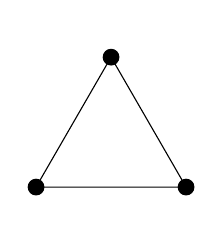
\begin{tikzpicture}
	\node (a) at (0cm,0.75cm) {};
	\node (b) at (0.866cm,-0.75cm) {};
	\node (c) at (-0.866cm,-0.75cm) {};
	\node [draw=none, fill=none] (1) at (0cm,-1cm) {};
	\node [draw=none, fill=none] (2) at (0cm,1cm) {};
	\draw (a) -- (b) -- (c) -- (a);
\end{tikzpicture}
$\qquad$
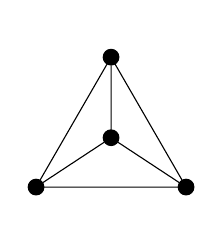
\begin{tikzpicture}
	\node (a) at (0cm,0.75cm) {};
	\node (b) at (0.866cm,-0.75cm) {};
	\node (c) at (-0.866cm,-0.75cm) {};
	\node (d) at (0cm, -0.18cm) {};
	\node [draw=none, fill=none] (1) at (0cm,-1cm) {};
	\node [draw=none, fill=none] (2) at (0cm,1cm) {};
	\draw (a) -- (b) -- (c) -- (d) -- (a);
	\draw (a) -- (c); \draw (b) -- (d);
\end{tikzpicture}
$\qquad$
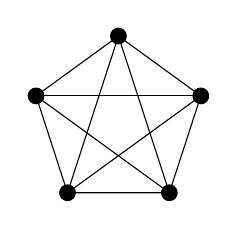
\begin{tikzpicture}
	\node (a) at (90:1cm) {};
	\node (b) at (162:1cm) {};
	\node (c) at (234:1cm) {};
	\node (d) at (306:1cm) {};
	\node (e) at (18:1cm) {};
	\node [draw=none, fill=none] (1) at (0cm,-1cm) {};
	\node [draw=none, fill=none] (2) at (0cm,1cm) {};
	\draw (a) -- (b); \draw (a) -- (c); \draw (a) -- (d); \draw (a) -- (e);
	\draw (b) -- (c); \draw (b) -- (d); \draw (b) -- (e); \draw (c) -- (d);
	\draw (c) -- (e); \draw (d) -- (e);
\end{tikzpicture}
$\qquad$
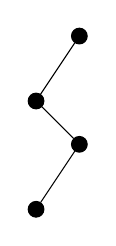
\begin{tikzpicture}
	\node (a) at (0.25cm,1cm) {};
	\node (b) at (-0.25cm,0.25cm) {};
	\node (c) at (0.25cm,-0.25cm) {};
	\node (d) at (-0.25cm,-1cm) {};
	\draw (a) -- (b) -- (c) -- (d);
\end{tikzpicture}
$\qquad$
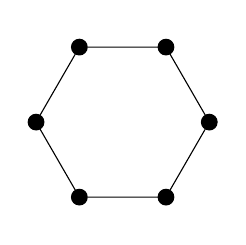
\begin{tikzpicture}
	\node (a) at (180:1cm) {};
	\node (b) at (120:1cm) {};
	\node (c) at (60:1cm) {};
	\node (d) at (0:1cm) {};
	\node (e) at (300:1cm) {};
	\node (f) at (240:1cm) {};
	\node [draw=none, fill=none] (1) at (0cm,-1cm) {};
	\node [draw=none, fill=none] (2) at (0cm,1cm) {};
	\draw (a) -- (b) -- (c) -- (d) -- (e) -- (f) -- (a);
\end{tikzpicture}

\caption{Drawings of $K_3$, $K_4$, $K_5$ (nonplanar), a length $4$ path, and a
	$6$-cycle.}
\end{center}
\end{figure}

A \textit{drawing} of a graph maps each vertex to a point in the
plane and each edge to a curve connecting its endpoints. A \textit{planar
embedding} is a drawing where edge curves intersect only at their
endpoints. We say a graph is \textit{planar} if it admits a planar embedding. A
planar graph together with a particular planar embedding is called a
\textit{plane graph}.

Let $G$ be a plane graph. A \textit{face} of $G$ is a maximal region
of the plane not containing any point used in the embedding. The unbounded face
is known as the \textit{outer face}. We will always refer to a face by the
subgraph of vertices and edges that lie on its border.

For brevity, we have
not fully formalized curves, regions, or borders. However, the
above definitions and results are fairly standard and may be found in many graph
theory texts, for example \cite{west}.

\begin{theorem}[Euler's Formula]
If $G$ is a connected plane graph with $n$ vertices, $m$ edges, and $f$ faces,
then $n-m+f=2$.
\end{theorem}

A simple corollary of Euler's Formula states that if $n\ge 3$, then $m\le 3n-6$.
A planar graph is said to be \textit{triangulated} if adding any new edge
results in a nonplanar graph. Triangulated plane graphs with $n\ge 3$ vertices
have exactly $3n-6$ edges.

A face is said to be a \textit{triangle} if it is a
$3$-cycle. It is easy to see that all faces in a triangulated
plane graph are triangles: if any face has more than three vertices then we may
add an edge curve connecting two face vertices without crossing existing edges.
Conversely if all faces in a plane graph are triangles, then it is triangulated.

\begin{comment}
\begin{figure}
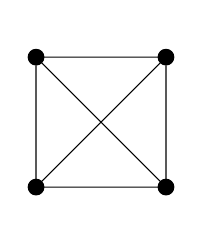
\begin{tikzpicture}
	\node (a) at (0.75cm,0.75cm) {};
	\node (b) at (0.75cm,-0.75cm) {};
	\node (c) at (-0.75cm,-0.75cm) {};
	\node (d) at (-0.75cm,0.75cm) {};
	\node [draw=none, fill=none] (1) at (0cm,-1cm) {};
	\node [draw=none, fill=none] (2) at (0cm,1cm) {};
	\draw (a) -- (b) -- (c) -- (d) -- (a);
	\draw (a) -- (c); \draw (b) -- (d);
\end{tikzpicture}
$\qquad$
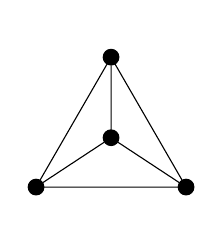
\begin{tikzpicture}
	\node (a) at (0cm,0.75cm) {};
	\node (b) at (0.866cm,-0.75cm) {};
	\node (c) at (-0.866cm,-0.75cm) {};
	\node (d) at (0cm, -0.18cm) {};
	\node [draw=none, fill=none] (1) at (0cm,-1cm) {};
	\node [draw=none, fill=none] (2) at (0cm,1cm) {};
	\draw (a) -- (b) -- (c) -- (d) -- (a);
	\draw (a) -- (c); \draw (b) -- (d);
\end{tikzpicture}

\caption{A nonplanar drawing and a planar embedding of $K_4$.}
\end{figure}
\end{comment}

If a plane graph has triangles for all but one face we shall say it is
\textit{weakly triangulated}. We will always assume the non-triangle face is the
outer face. A $2$-connected weakly triangulated plane graph has a cycle for its
nontriangle face.

Suppose $C$ is a cycle in a weakly
triangulated plane graph $G$. Then the subgraph consisting of $C$ and all interior
vertices and edges is denoted $\text{Int}(C)$. If $u,v \in V(C)$ then we denote
the $uv$-path in $C$ running clockwise around the cycle with $C[u,v]$. Finally,
if $u,v\in V(C)$ we call any edge $uv \in E(G)\setminus E(C)$ a \textit{chord} of
the cycle $C$.

A \textit{rotation scheme} for a graph is a cyclic ordering of the incident
edges around each vertex. Planar embeddings naturally induce a rotation
scheme by the counterclockwise order in which edge curves are positioned around
each vertex. In fact, with respect to graph algorithms, the induced rotation
scheme contains all the useful information of an embedding. Therefore, while we
may often visualize plane graphs with drawings, planar embeddings will always be
represented solely by their induced rotation scheme.

\section{A Brief History of Coloring Plane Graphs}

A $k$\textit{-coloring} of a graph maps each vertex to one of $k$ possible
colors. Equivalently, a $k$-coloring partitions the vertices of a graph into $k$
disjoint sets called \textit{color classes}. 
A coloring is \textit{proper} if no pair of adjacent vertices receive the same
color, or equivalently if the color classes all consist of nonadjacent vertices.

It is clear that not all planar graphs admit a proper $3$-coloring: the
complete graph on four vertices is planar and requires $4$ colors. Whether all
planar graphs admit a proper coloring with $4$ colors, the Four Color Problem,
remained one of the premier open questions in graph theory until it was verified
by Appel and Haken in 1976 \cite{appel1, appel2}.

A $(k,l)$-coloring, or a $k$-coloring with defect $l$, is a
$k$-coloring such that each vertex has at most $l$ same color neighbors.
Generalizations of proper colorings were first introduced in 1968 by Chartrand et al. in
\cite{chartrand}. Defective colorings in particular were introduced about
simultaneously around 1985 by Cowen et al. \cite{cowen}, Harary et al. \cite{jones}, and
Andrews et al. \cite{jacobson}. It was shown in \cite{cowen} that all
planar graphs admit a $(3,2)$-coloring.

A \textit{path $k$-coloring} is a
$k$-coloring such that the induced subgraph of each color class consists of one
or more disjoint paths. Note that path $k$-coloring is equivalent to
$(k,2)$-coloring with the added restriction that path coloring forbids cycles.
It was conjectured by Broere et. al. \cite{broere} that all planar graphs may
be path $3$-colored. In 1990 Poh \cite{poh} and Goddard \cite{goddard}
independently proved the conjecture. Planar graphs that do not admit a path $3$-coloring
were described by Chartrand et. al. \cite{kronk}, and thus the result is best possible.

Poh's proof is constructive and may easily be adapted to an algorithm for path
$3$-coloring plane graphs. Here we describe a naive version of Poh's algorithm,
as well as a modified algorithm that runs in $\mathcal{O}(n)$ time.

Let $G$ be a graph. A \textit{list assignment} for $G$ is a map $L$ assigning
each vertex $v\in V(G)$ a list of colors. Given a list assignment $L$ an
\textit{$L$-list-coloring} of $G$, first introduced
by Erd{\"o}s et al. in \cite{erdos}, maps each $v\in V(G)$ to a color in $L(v)$.
We say a graph $G$ is \textit{$k$-choosable} if given any list assignment $L$ such that
$|L(v)|\ge k$ for all $v\in V(G)$, $G$ admits a proper $L$-list-coloring.

In 1994 Thomassen \cite{thomassen} proved that if $G$ is planar, then $G$ is
$5$-choosable. A planar graph that is not $4$-choosable was
described by Voigt \cite{voigt} in 1993, so Thomassen's result is best possible.

We may equivalently define the properties \textit{$(k,l)$-choosable} and
\textit{path $k$-choosable}. In 1997 Hartman \cite{hartman} proved that all
planar graphs are path $3$-choosable. Hartman's result is best possible since
path $3$-coloring is a special case of path $L$-list-coloring with lists of size
$3$. In 1999 Hull and Eaton \cite{hull} and Skrekovski \cite{skrekovski}
independently proved that if $G$ is a planar graph, then $G$ is
$(3,2)$-choosable.

Hartman's proof provides a constructive procedure to find a path
$L$-list-coloring for a plane graph that has been given a list assignment $L$
with lists of size at least $3$. Interestingly, the proofs of Hartman and
Skrekovski follow the same coloring algorithm, and thus Skrekovski unknowingly
showed the stronger path $3$-choosability result. We describe an algorithm
based on Hartman and Skrekovski's work and show it runs in $\mathcal{O}(n)$
time.

\section{Graph Representations and Time Complexity}

Let $G$ be a plane graph. Vertices will be represented by integers, that is, we
shall assume $V(G)=\{0,1,\ldots,n-1\}$. We will always denote
number of vertices in $G$ with $n$ and the number of edges with $m$.

The input size for each algorithm, given input graph $G$, will be the
number of vertices $n$. However, since $G$ is a plane graph, if $n\ge 3$ then
$m\le 3n-6$. Thus $\mathcal{O}(m)= \mathcal{O}(n)$. Hence it is equivalent to
take the input size to be the number of edges $m$.

We assume an integer RAM model of computation in which integers require
fixed space and integer operations take constant time. The basic operation
for all time complexity discussions will therefore be a single memory reference
lookup, integer arithmetic operation, or integer comparison.

We will ignore the allocation of memory with respect to time complexity, such
as in the creation of arrays or other data structures. The operations
required to initialize elements in a structure are counted. In accordance
with these assumptions, inserting or removing an element in a linked list or at
the back of an array will require $\mathcal{O}(1)$ time.

Vertex properties will be stored in size $n$ arrays indexed by vertices. Thus accessing
or comparing vertex properties shall, in general, be constant time. Colors are assumed to be integers. A coloring of $G$ will thus be represented by
an integer vertex property.

For each $v\in V(G)$ we define a linked list called an
\emph{adjacency list} containing the neighbors of $v$ ordered according to
the rotation scheme of the embedding. The full plane graph $G$ may then
represented by a vertex property $\text{Adj}$ storing the adjacency list for
each vertex. That is, each vertex $v\in V(G)$ has the adjacency list $\text{Adj}[v]$.

We will sometimes wish for the ability to quickly find a neighbor $u$
in $v$'s adjacency list directly from $v$'s entry in $u$'s list. To allow this lookup in
$\mathcal{O}(1)$ time we will instead define a linked list of pairs $\text{Adj}[v]$ for
each $v\in V(G)$ called an \textit{augmented adjacency list}. Each node in the
list $\text{Adj}[v]$ will store a neighboring vertex $u$ as well as a reference
to the node for $v$ in $\text{Adj}[u]$.

An augmented adjacency list
representation of a graph $G$ may be constructed from a standard adjacency list
representation in $\mathcal{O}(m)$ time via the following algorithm due to 
Glenn Chappell \cite{chappell}.\\

\noindent\textbf{Algorithm 3.1.} (Augment Adjacency Lists)

\noindent\textbf{Input:} An adjacency list representation $\text{Adj}$ of a
graph $G$.

\noindent\textbf{Output:} An augmented adjacency list representation
$\text{Adj}'$ of $G$ with the neighbors of each vertex listed in the same order
as in $\text{Adj}$.

\noindent\textbf{Description:} We will begin by using $\text{Adj}$ to construct
an augmented adjacency list representation $\text{Adj}'$ of $G$ with the
reference portion of each node uninitialized.
Next we construct an array $\text{Wrk}[v]$ of size $\text{deg}(v)$ for each
$v\in V(G)$.

We fill in $\text{Wrk}$ as follows. For each $v$ from $0$ to $n-1$ let us walk
through $\text{Adj}'[v]$. At each neighbor $u$ in $\text{Adj}'[v]$ let
$r_{v,u}$ be the reference to $u$'s position in $\text{Adj}'[v]$ and append the
pair $(v,r_{v,u})$ to $\text{Wrk}[u]$.

After this process finishes each $u\in V(G)$ will have an array $\text{Wrk}[u]$
containing the pairs $(v,r_{v,u})$ for each neighbor $v$, sorted in ascending
order by the vertices $v$.

We will now initialize the references of each node of
the augmented adjacency lists.
Iterate through the vertices in descending order. Let $v$ be the current
vertex. For each 
$uw\in E(G)$ such that $u<w$ and $v<w$ we shall have initialized the reference
for $u$ in $\text{Adj}'[w]$ and the reference for $w$ in $\text{Adj}'[u]$. We
will also have removed the entry $(w,r_{w,u})$ from $\text{Wrk}[u]$. It remains
to handle edges $uv\in E(G)$ with $v>u$.

For each $v$ from $n-1$ to $0$ let us walk through $\text{Wrk}[v]$. For $i$ from
$1$ to $\text{deg}(v)$ take $(u,r_{u,v})=\text{Wrk}[v][i]$. Note $u<v$ by our
assumptions above. Moreover, $\text{Wrk}[u]$ contains no entries for neighbors
greater than $v$ so $(v,r_{v,u})$ is the last element of $\text{Wrk}[u]$. Thus
we may lookup $r_{v,u}$ to find $u$'s node in $\text{Adj}'[v]$ and initialize
the reference with $r_{u,v}$. We may similarly initialize the reference for
$v$'s node in $\text{Adj}'[u]$. Finally, we remove $(v,r_{v,u})$ from
$\text{Wrk}[u]$.

\noindent\textbf{Time Complexity:} For each edge $uv\in E(G)$, $u<v$, we make a
constant number of assignments to $\text{Adj}'$ and $\text{Wrk}$, two reference
lookups, and one entry removal from the back of $\text{Wrk}[u]$.
Therefore the overall complexity of the algorithm is $\mathcal{O}(m)$.\\

If $G$ is a planar graph without a given embedding we may still construct an
adjacency list representation of $G$, with neighbors simply listed in arbitrary
order. There exist numerous $\mathcal{O}(n)$ time algorithms to then reorder the
adjacency list representation of $G$ so that it corresponds to a valid planar
embedding of $G$ \cite{tarjan, lempel, boyer,
booth}. Additionally, there exist $\mathcal{O}(n)$ time algorithms to add edges
to the adjacency list representation in order to connect, $2$-connect, and
triangulate $G$, while maintaining planarity \cite{hagerup,reed,eswaran}.
Thus while the algorithms presented will often assume that input graphs are
triangulated and plane embedded, arbitrary planar graphs may be modified in
linear time to fit these criteria.

Some algorithm entries, for example \textit{Poh $3$-Coloring} (4.1), will
describe procedures on abstract graphs. Others, for example
\textit{Augment Adjacency Lists} (3.1), will describe algorithms
working with computer graph representations. We will provide time complexity
analysis for all algorithms working with concrete representations.

Each algorithm presented in this project will allocate some fixed number
of vertex properties, independent of the size of the graph. The size of all
other data structures constructed will be $\mathcal{O}(n)$ at all points during
the operation of each algorithm. Therefore the space complexity of every
algorithm is $\mathcal{O}(n)$.


\section{Path Coloring and the Poh Algorithm}

In this section we detail two algorithms for path $3$-coloring plane graphs. We
begin by describing the general procedure proposed by Poh \cite{poh}.\\

\noindent\textbf{Algorithm 4.1.} (Poh $3$-Coloring)

\noindent\textbf{Input:} A $2$-connected weakly triangulated plane graph $G$
with outer cycle $C=v_1v_2\ldots v_k$ and a $2$-coloring of $C$ such that the
color classes induce the paths $P=v_1v_2\ldots v_l$ and
$Q=v_{k}v_{k-1}\ldots v_{l+1}$.

\noindent\textbf{Output:} We find an extension of the $2$-coloring of $C$ to
a path $3$-coloring of $G$ such that no vertex in $C$ receives a same color
neighbor in $G-C$.

\noindent\textbf{Description:} If $G-C$ is empty there are no vertices remaining
to color. Otherwise the algorithm proceeds as follows.

\textit{Case 1:} Suppose there is a chord of $C$, that is, an edge
$v_iv_j\in E(G)\setminus E(C)$
with $i<j$. Since $P$ and $Q$ are induced paths it must be that $v_i\in P$ and
$v_j\in Q$. Let $C_1$ by the cycle consisting of $C[v_j,v_i]$ and the
edge $v_iv_j$, and $C_2$ the cycle consisting of $C[v_i,v_j]$ and the edge
$v_iv_j$. Observe $C_1$ and $C_2$ are each $2$-colored
such that each color class induces a path. Thus we may apply the algorithm to
path $3$-color $\text{Int}(C_1)$ and $\text{Int}(C_2)$. Since the subgraphs
$\text{Int}(C_1)$ and $\text{Int}(C_2)$ have only the vertices of the chord
$v_iv_j$ in common, the combined coloring forms a path $3$-coloring of $G$.

\textit{Case 2:} Suppose no chords of $C$ exist. Let $u$ be the neighbor of
$v_k$ immediately clockwise from $v_1$ and let $w$ be the neighbor of $v_l$
immediately clockwise from $v_{l+1}$. That is, $u,w\in\text{Int}(C)$ are the
unique, but possibly not distinct vertices such that the cycles $uv_1v_k$ and
$wv_lv_{l+1}$ are each faces of $G$.

Since $G$ is weakly triangulated, $G-C$ is nonempty, and $C$ has no chords, it
follows that $G-C$ is connected. Thus there exists a $uw$-path in
$G-C$. Let $T$ be the shortest such path, and note that therefore $T$ is
an induced path. Color $T$ with the remaining color not used on $P$ or $Q$.

Let $C_1$ be the cycle
consisting of $P$, $T$, and the edges $v_1u$ and $v_lw$. Similarly, let $C_2$ be
the cycle consisting of $T$, $Q$, and the edges $v_ku$ and $v_{l+1}w$. Then we
may apply the algorithm to path $3$-color $\text{Int}(C_1)$ and
$\text{Int}(C_2)$. Since $\text{Int}(C_1)$ and $\text{Int}(C_2)$ have only the
vertices of the path $T$ in common, the combined coloring forms a path
$3$-coloring of $G$.\\

\begin{figure}
\begin{center}
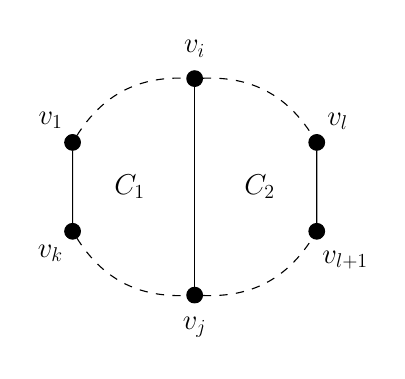
\begin{tikzpicture}
  \node (p0) [label=above left:$v_1$] at (160:1.5cm) {};
  \node (p1) [label=above:$v_i$] at (90:1.25cm) {};
  \node (pn) [label=above right:$v_l$] at (20:1.5cm) {};
  \node (q0) [label=below left:$v_{k}$] at (200:1.5cm) {};
  \node (q1) [label=below:$v_j$] at (270:1.25cm) {};
  \node (qn) [label=below right:$v_{l+1}$] at (340:1.5cm) {};
  \node (null) [draw=none, fill=none] at (270:1.75cm) {};
  
  \node (C1) [draw=none, fill=none] at (180:0.75cm) {$C_1$};
  \node (C2) [draw=none, fill=none] at (0:0.75cm) {$C_2$};
  
  \draw (p0) edge [bend left] (p1) [dashed];
  \draw (p1) edge [bend left] (pn) [dashed];
  \draw (q0) edge [bend right] (q1) [dashed];
  \draw (q1) edge [bend right] (qn) [dashed];
  \draw (p0) edge (q0);
  \draw (pn) edge (qn);
  \draw (p1) edge (q1);
\end{tikzpicture}
$\qquad$
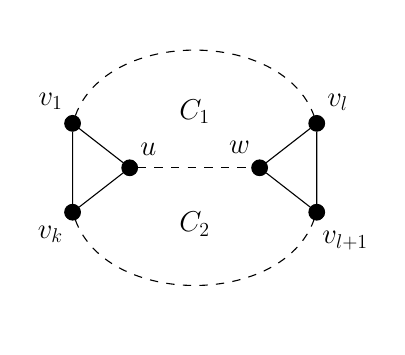
\begin{tikzpicture}
  \node (p0) [label=above left:$v_1$] at (160:1.5cm) {};
  \node (pn) [label=above right:$v_l$] at (20:1.5cm) {};
  \node (q0) [label=below left:$v_{k}$] at (200:1.5cm) {};
  \node (qn) [label=below right:$v_{l+1}$] at (340:1.5cm) {};
  \node (t0) [label=above right:$u$] at (180:0.75cm) {};
  \node (t1) [label=above left:$w$] at (0:0.75cm) {};
  \node (null) [draw=none, fill=none] at (270:1.75cm) {};
  
  \node (C1) [draw=none, fill=none] at (90:0.65cm) {$C_1$};
  \node (C2) [draw=none, fill=none] at (270:0.65cm) {$C_2$};
  
  \draw (p0) edge [bend left=70] (pn) [dashed];
  \draw (q0) edge [bend right=70] (qn) [dashed];
  \draw (p0) edge (q0);
  \draw (pn) edge (qn);
  \draw (p0) edge (t0);
  \draw (q0) edge (t0);
  \draw (pn) edge (t1);
  \draw (qn) edge (t1);
  \draw (t0) edge (t1) [dashed];
\end{tikzpicture}

\caption{The case of a chord (left) and the case no chord exists (right).}
\end{center}
\end{figure}

Given any plane graph $G$ we may add edges until it is triangulated. Observe
that any path coloring of $G$ with the additional edges is also a path coloring
of the original $G$. Therefore by path $2$-coloring the outer triangle we
may apply Poh's algorithm to path $3$-color $G$. This observation yields the
following result.

\begin{theorem}[Poh \cite{poh} and Goddard \cite{goddard}]
All planar graphs are path $3$-colorable.
\end{theorem}

\subsection{The Poh Algorithm with Breadth First Search}

In order to implement Poh's algorithm with adjacency lists there are two main
obstacles. First, we must have a method to efficiently represent colored paths,
as we will be recursively constructing paths and dividing the graph along them.
Second, we will need an efficient algorithm to locate the chords of $C$ and the
$uw$-path.

Let $G$ be a $2$-connected weakly triangulated plane graph with an adjacency
list representation. Each call of the algorithm will be provided with a cycle
$C$ in $G$ and produce a path $3$-coloring of $\text{Int}(C)$ according to the
specifications of Poh's algorithm.

To represent induced paths in $G$ we will simply use the color vertex property.
Suppose $P=v_1v_2\ldots v_k$ is an induced path in $G$ that has been colored
with $c_P$. Assume the coloring constructed so far is a path coloring. If
$v_i\in P$ then a neighbor $u$ of $v_i$ will have the color $c_P$ if and only if
$u\in P$, that is, $u=v_{i-1}$ or $u=v_{i+1}$. Therefore we may represent the
entire path by storing just the vertices $v_1$ and $v_k$. 

We will now describe the first version of Poh's algorithm on adjacency list
graphs, using a breadth first search to find induced paths and chords.\\

\noindent\textbf{Algorithm 4.2.} (Poh -- BFS)

\noindent\textbf{Assumptions:} Suppose $P=v_1v_2\ldots v_l$ and
$Q=v_kv_{k-1}\ldots v_{l+1}$ are induced
paths such that $C=v_1v_2\ldots v_k$ is a cycle. Additionally, assume each
path has been colored with a distinct color.

\noindent\textbf{Input:} The paths $P$ and $Q$, each represented by their
endpoints as described above.

\noindent\textbf{Output:} We find an extension of the $2$-coloring of $C$ to
a path $3$-coloring of $\text{Int}(C)$ such that
no vertex in $C$ receives a same color neighbor in $\text{Int}(C)-C$.

\begin{figure}
\begin{center}
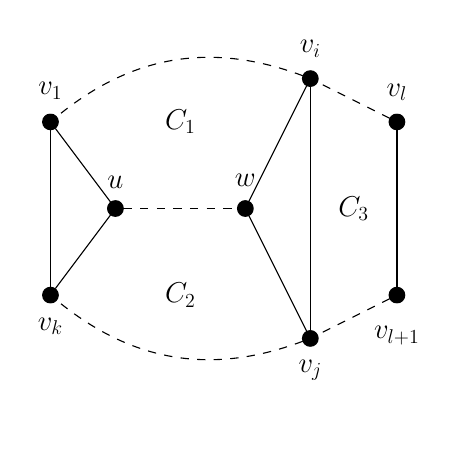
\begin{tikzpicture}
  \node (vl) [label=above:$v_l$] at (2cm, 1cm) {};
  \node (v1) [label=above:$v_1$] at (-2cm, 1cm) {};
  \node (vl1) [label=below:$v_{l+1}$] at (2cm, -1cm) {};
  \node (vk) [label=below:$v_k$] at (-2cm, -1cm) {};
  \node (w) [label=above:$w$] at (0.25cm, 0cm) {};
  \node (u) [label=above:$u$] at (-1.25cm, 0cm) {};
  \node (vi) [label=above:$v_i$] at (1cm, 1.5cm) {};
  \node (vj) [label=below:$v_j$] at (1cm, -1.5cm) {};
  
  \node (CP) [draw=none, fill=none] at (-0.5cm, 1cm) {$C_1$};
  \node (CQ) [draw=none, fill=none] at (-0.5cm, -1cm) {$C_2$};
  \node (Ci) [draw=none, fill=none] at (1.5cm, 0cm) {$C_3$};
  
  \node (null) [draw=none, fill=none] at (270:2.5cm) {};
  
  \draw (vl) edge (vi) [dashed];
  \draw (vi) edge [bend right] (v1) [dashed];
  \draw (vl1) edge (vj) [dashed];
  \draw (vj) edge [bend left] (vk) [dashed];
  \draw (vl) edge (vl1);
  \draw (v1) edge (vk);
  \draw (vi) edge (vj);
  \draw (v1) edge (u);
  \draw (vk) edge (u);

  \draw (u) edge (w) [dashed];
  \draw (vi) edge (w);
  \draw (vj) edge (w);
\end{tikzpicture}
$\qquad$
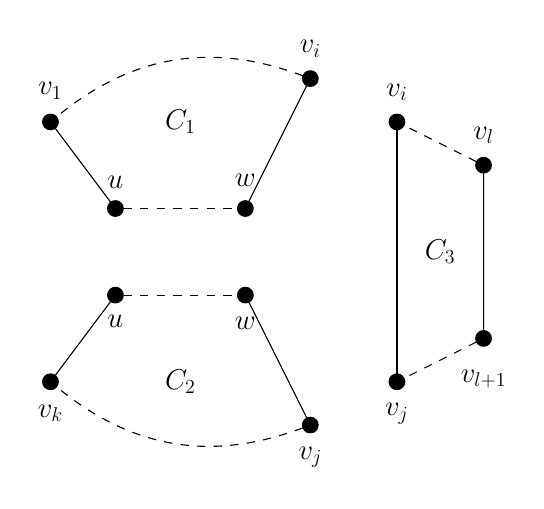
\begin{tikzpicture}
  \node (p0) [label=above:$v_l$] at (3cm, 1cm) {};
  \node (q0) [label=below:$v_{l+1}$] at (3cm, -1cm) {};
  \node (pi) [label=above:$v_i$] at (2cm, 1.5cm) {};
  \node (qj) [label=below:$v_j$] at (2cm, -1.5cm) {};
  
  \node (pi_1) [label=above:$v_i$] at (1cm, 2cm) {};
  \node (pn) [label=above:$v_1$] at (-2cm, 1.5cm) {};
  \node (t0) [label=above:$w$] at (0.25cm, 0.5cm) {};
  \node (t1) [label=above:$u$] at (-1.25cm, 0.5cm) {};
  
  \node (CP) [draw=none, fill=none] at (-0.5cm, 1.5cm) {$C_1$};
  \node (CQ) [draw=none, fill=none] at (-0.5cm, -1.5cm) {$C_2$};
  \node (Ci) [draw=none, fill=none] at (2.5cm, 0cm) {$C_3$};
  
  \node (qj_1) [label=below:$v_j$] at (1cm, -2cm) {};
  \node (qn) [label=below:$v_k$] at (-2cm, -1.5cm) {};
  \node (t0_1) [label=below:$w$] at (0.25cm, -0.5cm) {};
  \node (t1_1) [label=below:$u$] at (-1.25cm, -0.5cm) {};
  \node (null) [draw=none, fill=none] at (270:2.5cm) {};
  \draw (p0) edge (pi) [dashed];
  \draw (pi_1) edge [bend right] (pn) [dashed];
  \draw (q0) edge (qj) [dashed];
  \draw (qj_1) edge [bend left] (qn) [dashed];
  \draw (p0) edge (q0);
  \draw (pi) edge (qj);
  \draw (pn) edge (t1);
  \draw (qn) edge (t1_1);
  \draw (t1) edge (t0) [dashed];
  \draw (t1_1) edge (t0_1) [dashed];
  \draw (pi_1) edge (t0);
  \draw (qj_1) edge (t0_1);
\end{tikzpicture}

\caption{Dividing $G$ along the edge $v_iv_j$ and the $uw$-path.}
\end{center}
\end{figure}

\noindent\textbf{Description:} Locate the position of $v_k$ in
$\text{Adj}[v_1]$. Proceeding one vertex further in $\text{Adj}[v_1]$ gives us a
vertex $u$ such that the cycle $uv_1v_k$ is a triangle.

\textit{Case 1:} Suppose $u\in C$. If $u$ is in $P$, i.e. $u=v_2$, we apply the
algorithm to the paths $P-u$ and $Q$. Similarly if $w$ is in $Q$ we apply the
algorithm to $P$ and $Q-u$. In either case, if the two remaining paths each
consist of single vertex then there are no remaining uncolored vertices and we
terminate the algorithm.

\textit{Case 2:} Suppose $u\not\in C$. Perform a breadth first search from $u$
in $\text{Int}(C)-C$, that is, ignoring vertices in $C$. Terminate the search
when we reach a vertex
$w$ with neighbors $v_i\in P$ and $v_j \in Q$ such that $v_i$ is immediately
past $v_j$ in $\text{Adj}[w]$. Such a vertex must exist by the same argument
as in \textit{Poh $3$-Coloring} (4.1).
Backtracking from $w$ along the breadth first search and coloring vertices
produces an induced $uw$-path $T$, colored with the remaining color not used on
$P$ or $Q$.

Define the paths $P_1=v_1v_2\ldots v_i$, $P_2=v_ip_{i+1}\ldots v_l$,
$Q_1=v_kv_{k-1}\ldots v_j$, and $Q_2=v_jq_{j-1}\ldots v_{l+1}$. Observe we
have a cycle $C_1$ consisting of $P_1$, $T$, and the edges $v_1u$ and $v_iw$.
Similarly we have a cycle $C_2$ consisting of $T$, $Q_1$, and the edges $v_ku$
and $v_jw$. We apply the algorithm to $P_1$ and $T$ to color $\text{Int}(C_1)$
and similarly to $T$ and $Q_1$ to color $\text{Int}(C_2)$.

If $i=l$ and
$j=l+1$ we are done. Otherwise, we have the cycle $C_3$ consisting of $P_2$,
$Q_2$ and the edges $v_iv_j$ and $v_lv_{l+1}$, and we may apply the algorithm to
color $\text{Int}(C_3)$.

Note the combined coloring forms a path $3$-coloring of $\text{Int}(C)$ by the
same argument as in \textit{Poh $3$-Coloring} (4.1).

\begin{figure}
\begin{center}
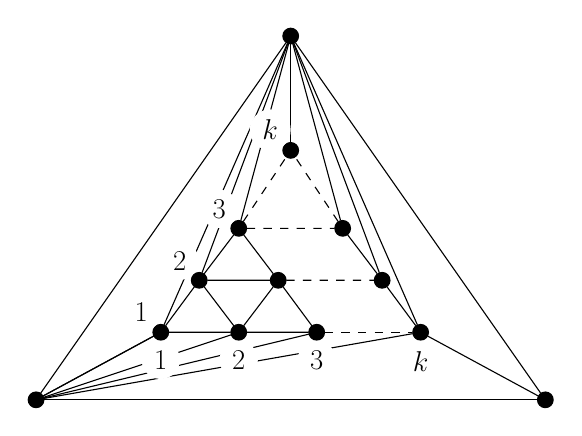
\begin{tikzpicture}[scale=1.2]
  \node (t1) at (0cm, 3.5cm) {};
  \node (t2) at (2.45cm, 0cm) {};
  \node (t3) at (-2.45cm, 0cm) {};
  
  \node (k1) [label=below:$1$, label=above left:$1$] at (-1.25cm, 0.65cm) {};
  \node (k2) [label=below:$2$]  at (-0.5cm, 0.65cm) {};
  \node (k3) [label=below:$3$]  at (0.25cm, 0.65cm) {};
  \node (kn) [label=below:$k$]  at (1.25cm, 0.65cm) {};
  
  \node (l1) [label=above left:$2$]  at (-0.88cm, 1.15cm) {};
  \node (l2) at (-0.12cm, 1.15cm) {};
  \node (ln) at (0.88cm, 1.15cm) {};
  
  \node (j1) [label=above left:$3$] at (-0.5cm, 1.65cm) {};
  \node (jn) at (0.5cm, 1.65cm) {};
  
  \node (p) [label=above left:$k$]  at (0cm, 2.4cm) {};
  
  \begin{pgfonlayer}{bg}
	  \draw (t1) edge (t2); \draw (t3) edge (t2); \draw (t1) edge (t3);
	  \draw (k1) edge (k2); \draw (k3) edge (k2);
	  \draw (k3) edge (kn) [dashed];
	  
	  \draw (l1) edge (l2);
	  \draw (l2) edge (ln) [dashed];
	  
	  \draw (j1) edge (jn) [dashed];
	  
	  \draw (j1) edge (p) [dashed];
	  \draw (jn) edge (p) [dashed];
	  
	  \draw (t1) edge (k1); \draw (t1) edge (kn);
	  \draw (t1) edge (l1); \draw (t1) edge (ln);
	  \draw (t1) edge (p);
	  \draw (t2) edge (kn); \draw (t3) edge (k1);
	  
	  \draw (k1) edge (l1); \draw (k2) edge (l1);
	  \draw (k2) edge (l2); \draw (k3) edge (l2);
	  \draw (kn) edge (ln);
	  
	  \draw (l1) edge (j1); \draw (l2) edge (j1);
	  \draw (jn) edge (ln);
	  
	  \draw (j1) edge (t1); \draw (jn) edge (t1);
	  
	  \draw (t3) edge (k1); \draw (t3) edge (k2);
	  \draw (t3) edge (k3); \draw (t3) edge (kn);
  \end{pgfonlayer}
  
\end{tikzpicture}

\caption{The collection of graphs $\{G_k\}_{k\in\mathbb{N}}$ on which Poh
performs poorly.}
\label{poh_example}
\end{center}
\end{figure}

\noindent\textbf{Complexity:} In the first step we rotate through
$\text{Adj}[v_1]$ to find $v_k$ and get an orientation within the graph. This
orientation must be performed at most once for each vertex, for a total of at
most $\sum_{v=0}^{n-1}\text{deg}(v)=2m$ operations.

In the next step we perform a breadth first search from the vertex $u$.
A breadth first search requires at most $m$ lookups. Moreover, the vertex will
$u$ will be colored following the search. Thus we perform at most one breadth
first search from each vertex, requiring at most $nm$ operations.
Therefore the complexity of the algorithm is $\mathcal{O}(2m + nm)
=\mathcal{O}(n^2)$.

We define the collection of graphs $\{G_k\}_{k\in\mathbb{N}}$, depicted in
Figure \ref{poh_example}. Let us fix $k\in\mathbb{N}$ and note $G_k$ has
$n=\frac{k^2+k}{2}+3$ vertices.

Suppose we apply \textit{Poh BFS} (4.2) to path $3$-color $G_k$.
Let the initial $2$-coloring of the outer triangle of $G_k$ assign the top
vertex a color distinct from the bottom two.
The $(k-i+1)$th recursive call will perform a breadth
first search visiting each vertex in a subgraph of size $\frac{i^2+i}{2}$,
hence requiring $\Theta(\frac{i^2+i}{2})$ operations. The total number
of operations required to path $3$-color $G_k$ is therefore
\[
    \Theta\left(\sum_{i=1}^k \frac{i^2+i}{2}\right)=\Theta(n^{3/2}).
\]
Thus the time complexity of the algorithm is $\Omega(n^{3/2})$. In
particular the algorithm is not linear.\\

\subsection{The Poh Algorithm in Linear Time}

Poh's proof requests that we find the shortest $uv$-path in $\text{Int}(C)$.
Therefore Poh's algorithm as written does not appear to admit a linear time
algorithm.

However, the correctness of Poh's algorithm does not require that $T$
be the shortest $uw$-path, only that $T$ be an induced $uw$-path. We will show
that Poh's algorithm is linear if we instead construct an induced $uw$-path
consisting of vertices in $G-C$ with at least one neighbor in the colored
path $P$.\\

\noindent\textbf{Algorithm 4.3.} (Poh -- Path Walk)

\noindent\textbf{Assumptions:} Assume $P=v_1v_2\ldots v_l$ and
$Q=v_kv_{k-1}\ldots v_{l+1}$ are induced paths, each colored with a distinct
color, such that $C=v_1v_2\ldots v_k$ is a cycle.

\noindent\textbf{Input:} The path $P$, represented by its endpoints, and the
color of the path $Q$.

\noindent\textbf{Output:} We find an extension of the $2$-coloring of $C$ to
a path $3$-coloring of $\text{Int}(C)$ such that
no vertex in $C$ receives a same color neighbor in $\text{Int}(C)-C$.

\noindent\textbf{Description:} 
We will iterate through the vertices of $P$ until we find a chord. All interior
vertices visited will be marked to indicate they have a neighbor in $P$. For
each $i$ from $1$ to $l$ let us walk through
$\text{Adj}[v_i]$ from $v_{i-1}$ to $v_{i+1}$, not including
$v_{i-1}$ and $v_{i+1}$.

Let $v$ be the current neighbor. If $v=v_j\in Q$ then $v_iv_j$ is a chord of $C$
and we stop. Otherwise $v\in \text{Int}(C)-C$ with the neighbor $v_i\in P$ and we
mark it.

Define the cycles $C_1$ and $C_2$ as usual by dividing $C$ along the chord
$v_iv_j$. Note $C_1$ is chordless as $P$ and $Q$ are induced paths
and $v_iv_j$ is the first chord of $C$ encountered. Apply \textit{Path Walk}
(4.3) to path $3$-color $\text{Int}(C_2)$. It remains to color
$\text{Int}(C_1)$.

If we never encountered a vertex in $\text{Int}(C)-C$ during our walk through
the neighbors of $v_1,\ldots,v_i$, then $\text{Int}(C_1)-C_1$ is empty and thus
$\text{Int}(C_1)$ is already colored. Otherwise let $u$ be the first such
neighbor encountered. Note $u$ is the unique vertex
such that $uv_1v_l$ is a face. We may therefore apply \textit{Path Trace} (4.4)
to path $3$-color $\text{Int}(C_1)$.

The combined coloring is a path $3$-coloring of $\text{Int}(C)$ by the
same argument as in \textit{Poh $3$-Coloring} (4.1).

\noindent\textbf{Complexity:} See \textit{Path Trace} (4.4).\\

\noindent\textbf{Algorithm 4.4.} (Poh -- Path Trace)

\noindent\textbf{Assumptions:} Let $P=v_1v_2\ldots v_l$ and
$Q=v_kv_{k-1}\ldots v_{l+1}$ be induced paths, each colored with a distinct
color, such that $C=v_1v_2\ldots v_k$ is a chordless cycle. In
addition, suppose $\text{Int}(C)-C$ is nonempty and all vertices in
$\text{Int}(C)- C$ with at least one neighbor in $P$ have been marked.

\noindent\textbf{Input:} The vertex $u\in \text{Int}(C)-C$ such that the cycle
$uv_1v_k$ is a face, as well as the respective colors of the paths $P$ and $Q$.

\noindent\textbf{Output:} We find an extension of the $2$-coloring of $C$ to a
path $3$-coloring of $\text{Int}(C)$ such that no vertex in $C$ receives a same
color vertex in $\text{Int}(C)-C$.

\noindent\textbf{Description:} Initialize $T$ as the path consisting of the
single vertex $u$, coloring $u$ with the remaining color. We will recursively
add vertices to $T$ until we reach the unique vertex $w$ such that $wv_lv_{l+1}$
is a face.

Suppose we have constructed the induced path $T=t_1t_2\ldots t_d$, such that
$t_1=u$ and each $t_i$ has at least one neighbor in $P$.
Iterate through $\text{Adj}[t_d]$,
starting from $t_{d-1}$. Let $v$ be the current neighbor. If $v$ has a neighbor
in $P$ we color $v$, assign $T=t_1\ldots t_dv$, and repeat the process with $v$ as
the new end vertex. If $v\in P$ it must be that $t_d=w$ and we are finished
constructing $T$. Otherwise ignore $v$ and move to the next neighbor.

Note the process above must terminate since each vertex in $T$ has at least
one neighbor in $P$.

Let $T=t_1t_2\ldots t_d$ be the path constructed above. Suppose $t_it_j$ is an
edge with $t_i,t_j\in T$, $i<j$. If $i=1$ let us define the vertex $t_0$ to be
$v_1$. Since each vertex in $T$ has a neighbor in
$P$, by planarity it must be that $t_j$ is between $t_{i-1}$ and $t_{i+1}$
counterclockwise in $\text{Adj}[t_i]$. But by the construction of
$T$, $t_{i+1}$ is the first neighbor of $t_i$ counterclockwise from $t_{i-1}$.
Thus $j=i+1$.

Therefore the only edges between vertices in $T$ are the edges $t_1t_2,\ldots,
t_{d-1}t_d$. So $T$ is an induced path.

We apply \textit{Path Walk} (4.3) to path $3$-color $\text{Int}(C_2)$. It remains
to color any uncolored vertices in $\text{Int}(C_1)$.

All vertices in $T$ have at least one neighbor in $P$. Therefore any uncolored
vertex in $\text{Int}(C_1)$ must lie in a path $2$-colored chordless cycle of
the form $v_iv_{i+1}\ldots v_jt_{p+1}t_p$ or $v_iv_{i+1}\ldots v_jt_p$.
We will use the following procedure to locate all such cycles that contain
uncolored vertices and color them using \textit{Path Trace} (4.4).

\begin{figure}
\begin{center}
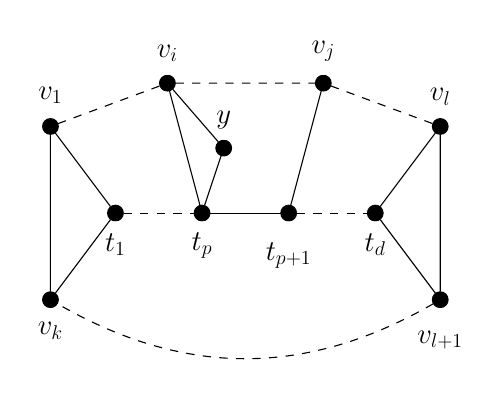
\begin{tikzpicture}
  \node (vl) [label=above:$v_l$] at (2.25cm, 1cm) {};
  \node (v1) [label=above:$v_1$] at (-2.25cm, 1cm) {};
  \node (vl1) [label=below:$v_{l+1}$] at (2.25cm, -1cm) {};
  \node (vk) [label=below:$v_k$] at (-2.25cm, -1cm) {};
  \node (w) [label=below:$t_d$] at (1.5cm, 0cm) {};
  \node (u) [label=below:$t_1$] at (-1.5cm, 0cm) {};
  \node (vi) [label=above:$v_i$] at (-0.9cm, 1.5cm) {};
  \node (vj) [label=above:$v_j$] at (0.9cm, 1.5cm) {};
  
  \node (tp) [label=below:$t_p$] at (-0.5cm, 0cm) {};
  \node (tp1) [label=below:$t_{p+1}$] at (0.5cm, 0cm) {};
  
  \node (y) [label=above:$y$] at (-0.25cm, 0.75cm) {};

  \draw (v1) edge (vi) [dashed];
  \draw (vi) edge (vj) [dashed];
  \draw (vj) edge (vl) [dashed];
  \draw (vl1) edge [bend left] (vk) [dashed];
  
  \draw (vl) edge (vl1);
  \draw (v1) edge (vk);
  
  \draw (v1) edge (u);
  \draw (vk) edge (u);

  \draw (vl) edge (w);
  \draw (vl1) edge (w);
  
  \draw (u) edge (tp) [dashed];
  \draw (tp) edge (tp1);
  \draw (tp1) edge (w) [dashed];
  
  \draw (tp) edge (vi);
  \draw (tp1) edge (vj);
  
  \draw (tp) edge (y);
  \draw (vi) edge (y);
\end{tikzpicture}
$\quad$
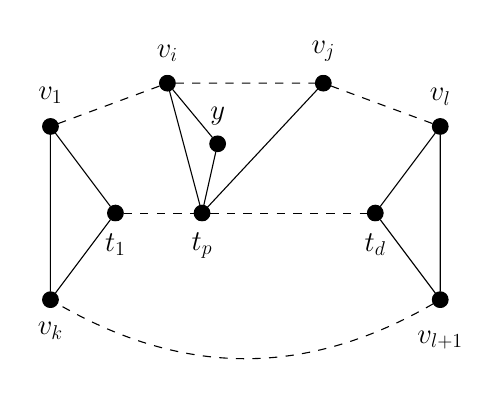
\begin{tikzpicture}
  \node (vl) [label=above:$v_l$] at (2.25cm, 1cm) {};
  \node (v1) [label=above:$v_1$] at (-2.25cm, 1cm) {};
  \node (vl1) [label=below:$v_{l+1}$] at (2.25cm, -1cm) {};
  \node (vk) [label=below:$v_k$] at (-2.25cm, -1cm) {};
  \node (w) [label=below:$t_d$] at (1.5cm, 0cm) {};
  \node (u) [label=below:$t_1$] at (-1.5cm, 0cm) {};
  \node (vi) [label=above:$v_i$] at (-0.9cm, 1.5cm) {};
  \node (vj) [label=above:$v_j$] at (0.9cm, 1.5cm) {};
  
  \node (tp) [label=below:$t_p$] at (-0.5cm, 0cm) {};
  
  \node (y) [label=above:$y$] at (-0.32cm, 0.8cm) {};

  \draw (v1) edge (vi) [dashed];
  \draw (vi) edge (vj) [dashed];
  \draw (vj) edge (vl) [dashed];
  \draw (vl1) edge [bend left] (vk) [dashed];
  
  \draw (vl) edge (vl1);
  \draw (v1) edge (vk);
  
  \draw (v1) edge (u);
  \draw (vk) edge (u);

  \draw (vl) edge (w);
  \draw (vl1) edge (w);
  
  \draw (u) edge (tp) [dashed];
  \draw (tp) edge (w) [dashed];
  
  \draw (tp) edge (vi);
  
  \draw (tp) edge (y);
  \draw (vi) edge (y);
  \draw (tp) edge (vj);
\end{tikzpicture}
\caption{Coloring vertices above $T$ in \textit{Path Trace} (4.4) case 1 (left),
case 2 (right).}
\end{center}
\end{figure}

For each $p$ from $1$ to $d$ let us iterate through
$\text{Adj}[t_p]$, starting with $t_{p+1}$. In the case $p=d$ we will define
$t_{p+1}=v_l$. Suppose we visit a neighbor $y\in \text{Int}(C_1)-C_1$ followed
counterclockwise by a neighbor $v_i\in P$. There are two possible cases.

\textit{Case 1:} Suppose none of the neighbors of $t_p$ between $t_{p+1}$ and
$v_i$ counterclockwise are in $P$. Let
$j$ be the smallest integer such that $t_{p+1}v_j$ is an edge, noting again
that $i<j$ by planarity. Note since $P$ is an induced path the cycle
$C_y=t_pv_iv_{i+1}\ldots v_jt_{p+1}$ is chordless by the our selection of $v_j$.
Thus we may apply \textit{Path Trace} (4.4) to color $\text{Int}(C_y)$ with the
vertex $y$ forming the face $yt_pv_i$.

\textit{Case 2:} Suppose we have previously visited a neighbor of $t_p$ in $P$,
and let $v_j\in P$ be the most recent such neighbor visited. Note by planarity
it must be that $i<j$. Note the cycle $C_y=v_iv_{i+1}\ldots v_jt_p$ is chordless
since $P$ is an induced path.
We may therefore apply \textit{Path Trace} (4.4) to color $\text{Int}(C_y)$ with
the vertex $y$ forming the face $yt_pv_i$.

\noindent\textbf{Complexity:} Let $G$ be a plane graph that has been colored
with Poh. Let $P$ be a path induced by the path $3$-coloring of $G$. Note each
vertex is in exactly one such path.

Let $v\in P$. We iterated through $\text{Adj}[v]$ exactly once during
\textit{Path Walk} (4.3). We iterated through $\text{Adj}[v]$ at most twice
during \textit{Path Trace} (4.4): once to locate
the starting neighbor, and once to find the next vertex to add to the path and
find uncolored vertices above $T$.

Thus the time complexity of the algorithm is
\[
    \mathcal{O}\left(\sum_{v=0}^{n-1}3\cdot\text{deg}(v)\right)
    =\mathcal{O}(6m)=\mathcal{O}(n).
\]
More specifically, it is $\Theta(n)$.



\section{Path List-Coloring and the Hartman-Skrekovski Algorithm}

In this section we describe an algorithm for path
list-coloring plane graphs with lists of size $3$. The following algorithm on
abstract graphs is due to the independent work of Hartman \cite{hartman} and
Skrekovski \cite{skrekovski}.

Note that the description of the algorithm given below is structured differently
than the descriptions given by both Hartman and Skrekovski. This restructuring is, in
many ways, less elegant than both original proofs, but helps illuminate how the
algorithm will operate on a graph with an adjacency list representation.\\

\noindent\textbf{Algorithm 5.1.} (Hartman-Skrekovski -- Path Color)

\noindent\textbf{Input:} Let $G$ be a $2$-connected weakly triangulated plane
graph with outer cycle $C=v_1v_2\ldots v_k$. Let $x=v_1$ and $y\in C-x$.
Suppose $L$ is a list assignment for $G$ such that
for each vertex $v\in G$
\[
    \begin{array}{ll}
	    |L(v)|\ge 1 & \text{if } v=x \text{ or } v=y;\\
	    |L(v)|\ge 2 & \text{if } v\in C-x-y;\\
	    |L(v)|\ge 3 & \text{otherwise.}
    \end{array}
\]
We will call $x$ and $y$ the \textit{fixed} vertices. Assume all vertices are
uncolored except for potentially $x$ and $y$. If $x$ or $y$ are colored assume
$L(x)$, $L(y)$ contain only the color they have been assigned. 

\noindent\textbf{Output:} A path $L$-list-coloring of $G$ such that the fixed
vertices $x$ and $y$ each receive at most one same color neighbor.

\noindent\textbf{Description:} If $x$ is already colored
let $c$ be the color of $x$. Otherwise select arbitrary $c\in L(x)$. We will 
construct an induced path $P$, colored with $c$, and consisting of vertices from
$C$. The path will begin at $x$ and proceed clockwise along the outer face a
far as possible towards $y$. Initialize $P$ to consist of the single vertex
$x$.

Suppose we have constructed an induced path $P=v_{j_1}v_{j_2}\ldots v_{j_l}$
with $1=j_1<j_2<\ldots<j_l< k$. Let us select the largest integer $i$ such
that $v_i\in C[v_{j_l},y]$ and $c\in L(v_i)$. If no such $i$ exists we have
finished constructing $P$. Otherwise we append $v_i$ to $P$ and repeat.

Let $L'$ be a list assignment for $G$ defined such that for $v\in G$
\[
	L'(v) = \begin{cases}
				\{c\}, & \text{ if } v\in P;\\
				L(v), & \ \text{otherwise}.
			\end{cases}
\]
Let $P=v_{j_1}v_{j_2}\ldots v_{j_l}$ be the path constructed above.
For each vertex in $v_{j_i}\in P$, color $v_i$ with $c$.

Suppose
$i\in\{1,\ldots,l-1\}$ such that $j_i+1<j_{i+1}$. We apply \textit{Remove Path}
(5.2) to path $L'$-list-color the subgraph bounded by the cycle consisting of
$C[v_{j_i},v_{j_{i+1}}]$ and the edge $v_{j_i}v_{j_{i+1}}$, with colored path
$v_{j_{i+1}}v_{j_i}$, and fixed vertices $v_{j_i+1}$ and $v_{j_{i+1}-1}$.

If $y\in P$ let us define $y'=v_{j_l+1}$, otherwise $y'=y$.
We may apply \text{Remove Path} (5.2) to path $L'$-list-color the
subgraph bounded by the cycle consisting of $P$ and $C[v_{j_l},v_{j_1}]$, with
colored path $P$, and fixed vertices $v_k$ and $y'$.

Pairwise all subgraphs above have only vertices in the path $P$ in common.
By \textit{Remove Path} (5.2), no vertex with a neighbor in $P$ will
receive the color $c$. Therefore the combined coloring is a path
$L$-list-coloring of $G$ such that $x,y$ receive at most one same color
neighbor.\\

\noindent\textbf{Algorithm 5.2.} (Hartman-Skrekovski -- Remove Path)

\noindent\textbf{Input:} Let $G$ be a $2$-connected weakly triangulated plane
graph with outer cycle $C=v_1v_2\ldots v_k$. Let $P=v_1v_2\ldots v_l$ be an
induced path in $C$. Let $x=v_k$ and $y\in C-P$. Let $L$ be a list
assignment for $G$ such that for $v\in G$
\[
    \begin{array}{ll}
        L(v)=\{c\} & \text{if } v\in P;\\
	    |L(v)|\ge 1 & \text{if } v=x \text{ or } v=y;\\
	    |L(v)|\ge 2 & \text{if } v\in C-P-x-y;\\
	    |L(v)|\ge 3 & \text{otherwise.}
    \end{array}
\]
Assume if $|L(x)|=1$ then $c\not\in L(x)$. Additionally, assume for every
$v\in C[v_{l+1},y]$, if $v$ has a neighbor in $P$ then $c\not\in L(v)$.

We will once again refer to $x$ and $y$ as fixed vertices, although in this
algorithm it may be the case that $x=y$. Assume all
vertices are uncolored except for potentially $x$ and $y$. If $x$ or $y$ are
colored assume $L(x)$, $L(y)$ contain only the color they have been assigned.

\noindent\textbf{Output:} A path $L$-list-coloring of $G$ such that $x$ and
$y$ each receive at most one same color neighbor, and no vertex in
$G-P$ with a neighbor in $P$ receives the color $c$. If $x=y$ then $x$ will
receive no same colored neighbors in $G$.

\noindent\textbf{Description:}
Note $G$ is $2$-connected and weakly triangulated. Thus to disconnect $G$ by
removing vertices from $C$ we would need to remove vertices
$v_i,v_j\in C$ such that $v_iv_j$ is a chord of $C$.
Observe $P$ is a subgraph of $C$ and an induced path in $G$, so no vertices in
$P$ induce a chord of $C$. So $G-P$ is connected.

\textit{Case 1:} Suppose there is a chord of $C$ with an endpoint in $P$. Let us
select the smallest $i\in\{1,\ldots,l\}$ and largest $j\in\{l+2,\ldots,k-1\}$
such that $v_i\in P$ and $v_iv_j$ is a chord of $C$. Let $C_1$ be the cycle
consisting of $C[v_j,v_i]$ and the edge $v_iv_j$. Similarly, let $C_2$ be the
cycle consisting of $C[v_i,v_j]$ and the edge $v_iv_j$. Let
$P_1=v_1v_2\ldots v_i$ and $P_2=v_iv_{i+1}\ldots v_l$.

\textit{Case 1.1:} Suppose $y\in C[v_{l+2},x]$ and $v_j\in C[v_{l+2},y]$.
Then $x,y\in C_1$. We will first apply \textit{Remove Path} (5.2) to path
$L$-list-color $\text{Int}(C_1)$ with the colored path $P_1$, and fixed vertices
$x$ and $y$. We then apply \textit{Remove Path} (5.2)
to path $L$-list-color $\text{Int}(C_2)$ with colored path $P_2$, and the single
fixed vertex $v_j$.

The subgraphs $\text{Int}(C_1)$ and $\text{Int}(C_2)$ have only the chord
$v_iv_j$ in common. The vertex $v_i$ is an endpoint of the colored path in both
$\text{Int}(C_1)$ and $\text{Int}(C_2)$. Thus $v_i$ will receive at most one
same color neighbor in each. Since $v_j$ is the single fixed vertex in
$\text{Int}(C_2)$, $v_j$ will receive no same color neighbors in
$\text{Int}(C_2)$. Thus the combined coloring is a path $L$-list-coloring of
$G$ with $x,y$ receiving the correct number of shared color neighbors.

\textit{Case 1.2:} Otherwise $v_j\in C[y,v_{k-1}]$, $v_j\ne y$. Again, we first
apply \textit{Remove Path} (5.2) to path $L$-list-color $\text{Int}(C_1)$ with
the colored path $P_1$, and fixed vertices $x$ and $v_j$.
We may then apply \textit{Remove Path} (5.2) to path $L$-list-color
$\text{Int}(C_2)$ with colored path $P_2$, and fixed vertices $v_j$ and $y$.

Again $\text{Int}(C_1)$ and $\text{Int}(C_2)$ have only the chord $v_iv_j$ in
common. In both $\text{Int}(C_1)$ and $\text{Int}(C_2)$ the vertex $v_j$ is
fixed vertex, and $v_i$ is an endpoint of the colored path. Therefore $v_i$ and
$v_j$ will both have at most one same color neighbor in each subgraph. Thus the
combined coloring is a path $L$-list-coloring of $G$ with $x,y$ receiving the
correct number of shared color neighbors.

\textit{Case 2:} Suppose there are no chords of $C$ with endpoints in $P$.
Let $L'$ be a list assignment for $G-P$ defined by
\[
	L'(v) = \begin{cases}
				L(v)\setminus\{c\}, & \text{if } v \text{ has at least one
				    neighbor in } P;\\
				L(v), & \ \text{otherwise}.
			\end{cases}
\]

\textit{Case 2.1:} Suppose $G-P$ is $2$-connected. Let $v\in G-P$.

Suppose $v$ is not on the outer face of $G-P$. Then $v$ has no neighbors in $P$
and $|L'(v)|=|L(v)|\ge 3$.

Suppose $v$ is on the outer face of $G-P$, $v\not\in C$. Then $v$ has at
least one neighbor in $P$ and $|L'(v)|\ge |L(v)|-1\ge 2$.

Finally, suppose $v\in C$. Since there are no chords of $C$ with endpoints in
$P$ the only vertices in $C-P$ with neighbors in $P$ are $x$ and $v_{l+1}$.
Recall we assumed that if $v\in C[v_{l+1},y]$ and $v$ has at least one neighbor
in $P$ then $c\not\in L(v)$. Thus if $v\ne x$, $v\ne y$, then
$|L'(v)|=|L(v)|\ge 2$. We ensured $c\not\in L(x)$ if $|L(x)|=1$. Thus if $v=x$
or $v=y$, $|L'(v)|\ge 1$.

Therefore $L'$ meets the requirements of \textit{Path Color}
(5.1) with fixed vertices $x$ and $y$. Moreover, by the definition of $L'$, in
a path $L'$-list-coloring of $G-P$ no vertex with a neighbor in $P$ will receive
the color $c$.

\textit{Case 2.1.1:} Suppose $x\ne y$. Then we may apply \textit{Path Color}
(5.1) to path $L'$-list-color $G-P$ with fixed vertices $x$ and $y$, the new
path starting at $x$.

\textit{Case 2.1.2:} Suppose $x=y$. If $x$ is uncolored select arbitrary
$c_x\in L'(x)$, color $x$ with $c_x$, and define $L'(x)=\{c_x\}$. Apply
\textit{Remove Path} (5.2) to path $L'$-list-color $G-P$
with the colored path consisting of the single vertex $x$, and the vertices
adjacent to $x$ on the outer cycle of $G-P$ as fixed vertices. This ensures $x$
receives no same colored neighbors in $G$.

\textit{Case 2.2:} Finally, if $G-P$ is not $2$-connected, then $G-P$ must be a
complete graph on one or two vertices. It is simple to check we may
$L'$-list-color $G-P$ such that the requirements hold.\\

Let $G$ be a plane graph and $L$ a list assignment such that $|L(v)|\ge 3$
for all $v\in G$. We may add edges to $G$ until it is triangulated. Then
we may apply \textit{Path Color} (5.1), with arbitrary fixed vertices, to
construct a path $L$-list-coloring. This yields the following result.

\begin{theorem}[Hartman \cite{hartman}]
All planar graphs are path $3$-choosable.
\end{theorem}

\subsection{The Hartman-Skrekovski Algorithm with Adjacency Lists}

In order to implement Hartman and Skrekovski's algorithm with adjacency lists
there are two main challenges. First, we must be able to remove paths and
locate the subgraphs for recursive calls. Second, we must be able to track the
location of vertices on the outer face with respect to the fixed vertices
$x$, and $y$. For example: when adding a vertex to the path
$P=v_{j_1}v_{j_2}\ldots v_{j_l}$ in \textit{Path Color} (5.1), we need to know
which neighbors of $v_{j_l}$ lie in $C[v_{j_l},y]$.

For now, let us assume we have solved the second challenge described above. That
is, given vertices $u,v,w\in C$, assume we can determine whether $v\in C[u,w]$
in $\mathcal{O}(1)$ time.

Let $G$ be a $2$-connected weakly triangulated plane graph with an augmented
adjacency list representation. Just as in Poh's algorithm, each call will be
provided with a cycle $C=v_1v_2\ldots v_k$ in $G$. The
job of a particular recursive call is then to color the subgraph $\text{Int}(C)$
such that the requirements of the Hartman-Skrekovski algorithm hold.

We will provide each vertex in $G$ with a boolean vertex property to represent
its state. All vertices in $C$ will be have a state indicating they are on the
outer face, and likewise vertices in $\text{Int}(C)-C$ will have a state
indicating they are not in $C$.

The list assignment $L$ will be represented by vertex property storing a linked
list of colors $L[v]$ for each $v\in G$. We will denote the number of colors
in the linked list by $|L[v]|$. We will produce a coloring of $G$ by reducing
the size of each color list to one. Thus we consider a vertex $v$
colored if $|L[v]|=1$.

For each vertex $v_i\in C$ we will store a vertex property $\text{Nbr}[v_i]$
called a \textit{neighbor range}. The neighbor range of $v_i$ will contain a pair of
references to nodes in $\text{Adj}[v_i]$, that is $\text{Nbr}[v_i]=(r_1,r_2)$.
The first reference $r_1$ will point to the
node for $v_{i-1}$ in $\text{Adj}[v_i]$ and the reference $r_2$ will point to
the node for $v_{i+1}$.

Neighbor ranges provide immediate access to the preceding and subsequent
vertices of $v_i$ in $C$. Additionally, they give start and stop nodes in
$\text{Adj}[v_i]$ for the list of neighbors of $v_i$ that are contained in the
subgraph $\text{Int}(C)$.\\

\noindent\textbf{Algorithm 5.3.} (Hartman-Skrekovski -- Path Color)

\noindent\textbf{Assumptions:} Suppose $C=v_1v_2\ldots v_k$ is a cycle, $x=v_1$,
and $y\in C-x$. Assume for each $v\in \text{Int}(C)$
\[
    \begin{array}{ll}
	    |L[v]|\ge 1 & \text{if } v=x \text{ or } v=y;\\
	    |L[v]|\ge 2 & \text{if } v\in C-x-y;\\
	    |L[v]|\ge 3 & \text{otherwise.}
    \end{array}
\]
Assume the vertices of
$\text{Int}(C)$ have been assigned according to whether they are in $C$ or
$\text{Int}(C)-C$. Finally, assume for each $v_i\in C$ we have constructed
$\text{Nbr}[v_i]$ as described above.

\noindent\textbf{Input:} The fixed vertices $x$ and $y$.

\noindent\textbf{Output:} A path $L$-list-coloring of $\text{Int}(C)$ such that
$x$ and $y$ each receive at most one same color neighbor.

\noindent\textbf{Description:} If $x$ is colored let $c$ be the color of $x$.
Otherwise let $c$ be the first color in $L[x]$ and assign
$L[x]=\{c\}$.

Initialize $P$ to contain the single vertex $x$. We will now
append vertices to $P$ following the procedure of \textit{Path Color} (5.1).

Suppose we have constructed an induced path $P=v_{j_1}v_{j_2}\ldots v_{j_l}$
with $1=j_1<j_2<\ldots<j_l< k$. Let $v=v_{j_l}$ be the last vertex added to $P$.
Let us iterate through $\text{Adj}[v]$ counterclockwise from $v_{j_{l-1}}$, if
$l=1$ start from $v_k$. Let $u$ be the current neighbor.

\textit{Case 1:} If $u\not\in C[v,y]$ or $c\not\in L(u)$ then we ignore $u$ and
continue to the next vertex in $\text{Adj}[v]$.

\textit{Case 2:} Suppose $u=v_i\in C$,
$u\in C[v,y]$, and $c\in L(u)$, that is, suppose we may add $u$ to $P$.
There are two cases to consider.

\textit{Case 2.1:} Suppose the start node of $\text{Nbr}[u]$ is not $v$. Then
$u\ne v_{j_l +1}$. Let $\text{Nbr}[u]=(r_1,r_2)$ and
$\text{Nbr}[v_{j_l}]=(s_1,s_2)$. Let $r_v$ be the reference to the node for
$v$ in $\text{Adj}[u]$ and $s_u$ be the reference to the node for $u$ in
$\text{Adj}[v]$.

Let us assign $\text{Nbr}[u]=(r_1,r_v)$ and $\text{Nbr}[v]=(s_u,s_2)$. We will
then call \textit{Remove Path} (5.4) on the cycle consisting of $C[v,u]$ and the
edge $uv$, with colored path $uv$, and fixed vertices $v_{i-1}$ and
$v_{j_l+1}$.

We then assign $\text{Nbr}[u]=(r_v,r_2)$ and $\text{Nbr}[v]=(s_1,s_u)$. Finally,
color $u$ with $c$, assign $L[u]=\{c\}$, append $u$ to $P$, and attempt to
continue the path from $u$.

\textit{Case 2.2:} Suppose the start node of $\text{Nbr}[u]$ is $v$. Then we may
color $u$ with $c$, assign $L[u]=\{c\}$, append $u$ to $P$, and attempt to
continue the path from $u$.

Let $P=v_{j_1}v_{j_2}\ldots v_{j_l}$ be the path constructed above.
If $y\in P$ let us define $y'=v_{j_l+1}$, otherwise $y'=y$.
We may finally apply \text{Remove Path} (5.4) to the cycle formed by $P$ and
$C[v_{j_l},v_{j_1}]$, with colored path $P$, and fixed
vertices $v_k$ and $y'$.

\noindent\textbf{Complexity:} See \textit{Remove Path} (5.4).\\

\noindent\textbf{Algorithm 5.4.} (Hartman-Skrekovski -- Remove Path)

\noindent\textbf{Assumptions:} Suppose $C=v_1v_2\ldots v_k$ is a cycle. Let
$P=v_1v_2\ldots v_l$ be an induced path in $C$ colored with some color $c$. Let
$y\in C-P$ and $x\in C[y,v_k]$. Let $L$ be a list assignment for $G$ such that
for each $v\in G$
\[
    \begin{array}{ll}
        L[v]=\{c\} & \text{if } v\in P;\\
	    |L[v]|\ge 1 & \text{if } v=x \text{ or } v=y;\\
	    |L[v]|\ge 2 & \text{if } v\in C-P-x-y;\\
	    |L[v]|\ge 3 & \text{otherwise.}
    \end{array}
\]
Assume for every $v\in C[x,v_k]$, $c\not\in L(v)$. Additionally, assume for
every $v\in C[v_{l+1},y]$, if $v$ has a neighbor in $P$ then $c\not\in L(v)$.

\noindent\textbf{Input:} The vertices $v_1$, $x$, and $y$.

\noindent\textbf{Output:} A path $L$-list-coloring of $G$ such that $x$ and
$y$ each receive at most one same color neighbor, and no vertex in
$G-P$ with a neighbor in $P$ receives the color $c$. If $x=y$ then $x$ will
receive no same colored neighbors in $G$.

\begin{comment}
\begin{figure}
\begin{center}
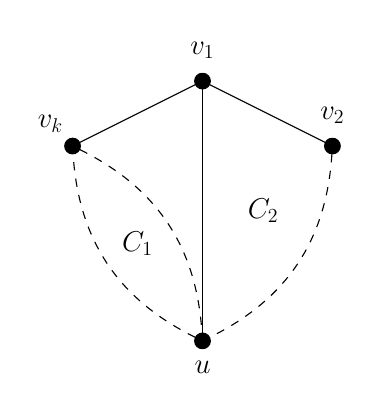
\begin{tikzpicture}
  \node (c_n) [label=above left:$v_k$, fill] at (-1.5cm, 1.25cm) {};
  \node (p) [label=above:{$v_1$}] at (0cm, 2cm) {};
  \node (p_label) [draw=none, scale=0.8] at (0cm, 2cm) {};
  \node (c_1) [label=above:$v_2$] at (1.5cm, 1.25cm) {};
  \node (c_i) [label=below:$u$] at (0cm, -1cm) {};
  \node (G_0) [draw=none, fill=none] at (-0.75cm, 0.12cm) {$C_1$};
  \node (G_1) [draw=none, fill=none] at (0.7cm, 0.5cm) {$C_2$};
  
  \draw (c_i) edge [bend left] (c_n) [dashed];
  \draw (c_n) edge [bend left] (c_i) [dashed];
  \draw (c_n) edge (p);
  \draw (p) edge (c_1);
  \draw (p) edge (c_i);
  \draw (c_1) edge [bend left] (c_i) [dashed];
\end{tikzpicture}
\end{center}

\caption{The cycles $C_1$ and $C_2$.}
\end{figure}
\end{comment}

\noindent\textbf{Description:} We will remove the path $P$ one vertex at a
time. In this call we will be ``removing" edges around $v_1$, by updating
$\text{Nbr}[v]$ to exclude them. We will completely removing $v_1$ from
$\text{Int}(C)$ if there are no chords $v_1v_i$ of $C$.

Let us iterate counterclockwise through $\text{Adj}[v_1]$ beginning from $v_k$.
Let $u$ be the current neighbor of $v_1$.

\textit{Case 1:} Suppose $u\not\in C$. Look through $L[u]$ and remove the color
$c$ if it exists. After removing $v_1$, $u$ will be on the
outer face. Thus we set the state of $u$ to indicate it is
on the outer face. Construct $\text{Nbr}[u]=(r_1,r_2)$ such that
$r_1$ is a reference to the node immediately prior to $v_1$ in $\text{Adj}[u]$
and $r_2$ is a reference to the node immediately subsequent to $v_1$.

\textit{Case 2:} Suppose $u\in C$. There are several cases to consider.

\textit{Case 2.1:} Suppose $u=v_k$. Let $\text{Nbr}[u]=(r_1,r_2)$. By our
assumptions $r_2$ is a reference to the node for $v_1$ in $\text{Adj}[u]$.
Reassign $r_2$ to be a reference to the node immediately prior to $v_1$ in
$\text{Adj}[u]$. This removes $v_1$ from the set of neighbors of $u$ contained
in the cycle.

\textit{Case 2.2:} Suppose $u\ne v_k$. In this case the edge $v_1u$ is either a
chord of $C$ or $u=v_2$. Let $N$ be the $v_ku$-path consisting of the neighbors
of $v_1$. Let $C_1$ be the cycle consisting of $N$ and $C[u,v_k]$. If $u\ne v_2$
let $C_2$ be the cycle consisting of $C[v_1,u]$ and the edge $v_1u$.

Let $\text{Nbr}[u]=(r_1,r_2)$ and
$\text{Nbr}[v]=(s_1,s_2)$. Let $r_v$ be the reference to the node for
$v$ in $\text{Adj}[u]$ and $s_u$ be the reference to the node for $u$ in
$\text{Adj}[v]$.

In all cases below, before we apply an algorithm to color
$\text{Int}(C_1)$ we will assign $\text{Nbr}[u]=(r_v,r_2)$ and $\text{Nbr}[v]=
(s_1,s_v)$. Similarly, before applying an algorithm to color $\text{Int}(C_2)$
we will assign $\text{Nbr}[u]=(r_1,r_v)$ and $\text{Nbr}[v]=(s_u,s_2)$.

We will now path $L$-list-color $\text{Int}(C_1)$ and, if $u\ne v_2$,
$\text{Int}(C_2)$. There are several cases to consider.

\begin{figure}
\begin{center}
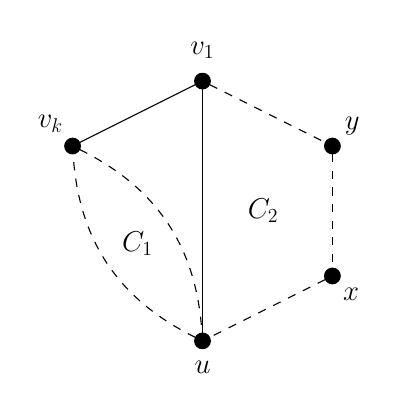
\begin{tikzpicture}
  \node (c_n) [label=above left:$v_k$, fill] at (-1.5cm, 1.25cm) {};
  \node (p) [label=above:{$v_1$}] at (0cm, 2cm) {};
  \node (y) [label=above right:$y$] at (1.5cm, 1.25cm) {};
  \node (x) [label=below right:$x$] at (1.5cm, -0.25cm) {};
  \node (c_i) [label=below:$u$] at (0cm, -1cm) {};
  \node (G_0) [draw=none, fill=none] at (-0.75cm, 0.12cm) {$C_1$};
  \node (G_1) [draw=none, fill=none] at (0.7cm, 0.5cm) {$C_2$};
  \node (null) [draw=none,fill=none] at (270:1.5cm) {};
  
  \draw (c_i) edge [bend left] (c_n) [dashed];
  \draw (c_n) edge [bend left] (c_i) [dashed];
  \draw (c_n) edge (p);
  \draw (p) edge (c_i);
  \draw (p) edge (y) [dashed];
  \draw (y) edge (x) [dashed];
  \draw (x) edge (c_i) [dashed];
\end{tikzpicture}
$\quad$
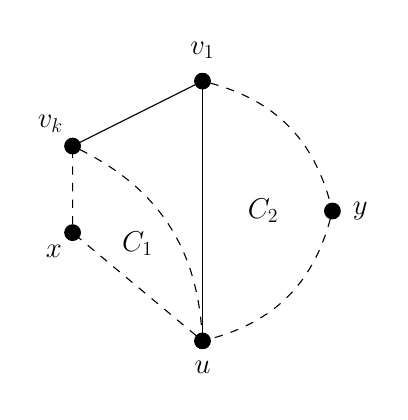
\begin{tikzpicture}
  \node (c_n) [label=above left:$v_k$, fill] at (-1.5cm, 1.25cm) {};
  \node (p) [label=above:{$v_1$}] at (0cm, 2cm) {};
  \node (x) [label=below left:$x$, fill] at (-1.5cm, 0.25cm) {};
  \node (y) [label=right:$y$, fill] at (1.5cm, 0.5cm) {};
  \node (c_i) [label=below:$u$, fill] at (0cm, -1cm) {};
  \node (G_0) [draw=none,fill=none] at (-0.75cm, 0.12cm) {$C_1$};
  \node (G_1) [draw=none,fill=none] at (0.7cm, 0.5cm) {$C_2$};
  \node (null) [draw=none,fill=none] at (270:1.5cm) {};
  
  \draw (c_i) edge (x) [dashed];
  \draw (x) edge (c_n) [dashed];
  \draw (c_n) edge [bend left] (c_i) [dashed];
  \draw (c_n) edge (p);
  \draw (p) edge (c_i);
  \draw (p) edge [bend left] (y) [dashed];
  \draw (y) edge [bend left] (c_i) [dashed];
\end{tikzpicture}
$\quad$
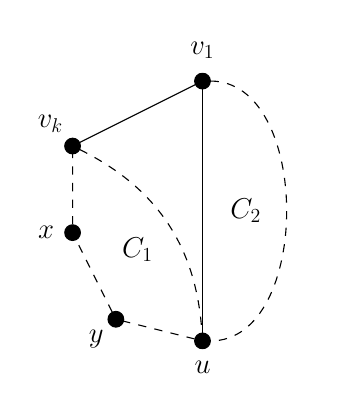
\begin{tikzpicture}
  \node (c_n) [label=above left:$v_k$, fill] at (-1.5cm, 1.25cm) {};
  \node (p) [label=above:{$v_1$}] at (0cm, 2cm) {};
  \node (x) [label=left:$x$, fill] at (-1.5cm, 0.25cm) {};
  \node (y) [label=below left:$y$, fill] at (-1cm, -0.75cm) {};
  \node (c_i) [label=below:$u$, fill] at (0cm, -1cm) {};
  \node (G_0) [draw=none,fill=none] at (-0.75cm, 0.05cm) {$C_1$};
  \node (G_1) [draw=none,fill=none] at (0.5cm, 0.5cm) {$C_2$};
  \node (null) [draw=none,fill=none] at (270:1.5cm) {};
  
  \draw (c_i) edge (y) [dashed];
  \draw (y) edge (x) [dashed];
  \draw (x) edge (c_n) [dashed];
  \draw (c_n) edge [bend left] (c_i) [dashed];
  \draw (c_n) edge (p);
  \draw (p) edge (c_i);
  \draw (p) edge [bend left=90] (c_i) [dashed];
\end{tikzpicture}
\end{center}

\caption{From left to right: case 2.2.1, case 2.2.2, and case 2.2.3.}
\end{figure}

\textit{Case 2.2.1:} Suppose $u\in C[x,v_1]$. Note in this case it must be that
$u\ne v_2$. We will first apply \textit{Remove Path} (5.4) to path $L$-list-color
$\text{Int}(C_2)$ with fixed vertices $x$ and $y$. Note this colors the vertex
$u$. We will apply \textit{Remove Path} (5.4) with colored path consisting of
just the vertex $u$, and the vertices immediately adjacent to $u$ on $C_1$ as
the fixed vertices. This ensures $u$ receives no same color neighbors in
$\text{Int}(C_1)$. 

\textit{Case 2.2.2:} Suppose $u\in C[y,x]$, $u\ne y$. Again it must be that
$u\ne v_2$. We apply \textit{Color Path} (5.3) to path $L$-list-color
$\text{Int}(C_1)$ with fixed vertices $x$ and $u$, the new path starting at $x$.
Next we apply \textit{Remove Path} (5.4) to $\text{Int}(C_2)$ with fixed
vertices $u$ and $y$.

\textit{Case 2.2.3:} Suppose $u\in C[v_1,y]$, $u\ne v_2$. We apply
\textit{Color Path} (5.3) to path $L$-list-color $\text{Int}(C_1)$ with fixed
vertices $x$ and $y$, the new path starting at $x$. We then apply \textit{Remove
Path} (5.4) to path $L$-list-color $\text{Int}(C_2)$ with the single fixed 
vertex $u$. This ensures $u$ receives no same color neighbors in
$\text{Int}(C_2)$.

\textit{Case 2.2.4:} Suppose $u= v_2$. If $c\in L[u]$ then $u$ is a path vertex
and we apply \textit{Remove Path} (5.4) to path $L$-list-color $\text{Int}(C_1)$
with fixed vertices $x$ and $y$. Otherwise, we have reached the end of the path.
We apply \textit{Color Path} (5.3) to $\text{Int}(C_1)$ with fixed vertices $x$
and $y$, the new path starting from $x$.

\noindent\textbf{Complexity:} Let $v\in G$. We iterate through $\text{Adj}[v]$
at most once during \textit{Color Path} (5.3) when looking for the next vertex
to add to the path containing $v$. In \textit{Remove Path} (5.4) we iterate through
$\text{Adj}[v]$ exactly once. We also iterate through $\text{Adj}[v]$ once
when we initially construct $\textit{Nbr}[v]$ to locate start and stop nodes.
Therefore the overall complexity of the algorithm is
\[
    \mathcal{O}\left(\sum_{v=0}^{n-1}3\cdot\text{deg}(v)\right)
        =\mathcal{O}(6m)=\mathcal{O}(n).
\]
More specifically, it is $\Theta(n)$.

\subsection{Tracking Vertices on the Outer Cycle}

The Hartman-Skrekovski algorithm described in the previous section relied on the
assumption that we could immediately
know the relative location of vertices on the outer cycle. In
\textit{Path Color} (5.3) we assumed we could determine
whether a given vertex $u\in C$ was in the path $C[v,y]$, where $v$ was the
last vertex added to our colored path. Additionally, in \textit{Remove Path}
(5.4) we assumed for $u\in C$ we could determine whether $u$ was in $C[x,v_l]$,
$C[y,x]$, or $C[v_1,y]$. We will now describe how this check may be accomplished
in $\mathcal{O}(1)$ time.

Let us define an integer vertex property to store a location mark for each
vertex on the outer cycle. Assume we are given the input for \textit{Remove
Path} (5.4). Also assume vertices in $C[v_1,y]$ have been assigned the mark $n_1$,
vertices in $C[y,x]$ have the mark $n_2$, and vertices in $C[y,v_k]$ have
the mark $n_3$.

Let us iterate through $\text{Adj}[v_1]$ starting from $v_k$ as in (5.4). Let
$u$ be the current neighbor. If $u\not\in C$ we will assign $u$ the mark $n_1$.
This is because $u$ will be in $C_1[x,v_2]$ if there are no chords $v_1v_i$.

Now suppose we reach the end of the colored path, or we hit a chord $v_1u$ with
$u\in C[v_1,x]$. Then in the subsequent call to \textit{Color Path} (5.3) on
$\text{Int}(C_1)$ we will need to treat vertices marked $n_1$ and $n_2$ as the
same segment, since $C_1[x,y]$ consists of both $C_1[x,v_k]$ and $C_1[u,y]$.
One solution is to walk along $C_1$ and remark vertices, but this is very
inefficient. Another solution is to simply compare with both marks to check
whether a vertex is in $C_1[x,y]$. However, we will be drawing further colored
paths and generating further marks, hence the collection of marks to compare
may grow very large.

Our solution is to use a disjoint set structure to compare location marks. All
marks begin as singleton sets. To join the segments marked with $n_1$ and
$n_2$ above we may simply perform a union operation in the disjoint set structure.

The mark $n_1$ for the segment $C_1[x,v_k]$ will always be a singleton set in the
disjoint set structure. This is because the only vertices marked with $n_1$ are
vertices that have been added to the outer face while removing vertices from the
colored path. Thus in each union operation performed at least one of the two sets
is always a singleton. Because of this, standard disjoint set optimizations
allow set lookups in constant time. Therefore performing
$\mathcal{O}(n)$ make set, union, and lookup operations in the disjoint set
structure requires $\mathcal{O}(n)$ time. Hence the overall performance of the
algorithm remains linear.

For full details on managing location marks and disjoint set operations, see the
provided C++ implementation.

\section{Path $3$-Coloring and Path List-Coloring in C++}

In this section we detail the C++ implementation of each algorithm above.
Instructions for using each algorithm are provided, as well as brief examples.

The Boost Graph Library (BGL) \cite{boost} details a generic interface for working
with graphs, as well as numerous data structures and algorithms. We will begin
with a brief introduction to the BGL. Then we will
discuss implementing the Poh and Hartman-Skrekovski algorithms using BGL
abstractions.

We will assume familiarity with the C++ language and the
C++ Standard Template Library (STL). Full hyperlinked documentation is
available with the project source code at
\url{https://github.com/permutationlock/path_coloring_bgl},
with links to the relevant Boost and STL concepts.

\subsection{The Boost Graph Library}

The BGL provides several abstract concepts for graph data structures.
The basic \texttt{Graph} concept requires that a vertex and edge type to be
defined, as well as a few properties such as whether the graph is directed or
undirected. The \texttt{VertexListGraph} and \texttt{EdgeListGraph} refine this
concept to additionally require an interface to iterate over the vertex and
edge sets, respectively. The \texttt{VertexAndEdgeListGraph} concept simply
combines the two refinements.

Although other concepts exist such as
\texttt{AdjacencyGraph}, we will only require that input graphs model
\texttt{VertexListGraph} or \texttt{VertexAndEdgeListGraph}. The
\texttt{Adjacency{\allowbreak}Graph} concept might seem like an obvious choice,
but we follow the BGL's decision and represent the rotation scheme for planar
embeddings as an exterior property map. Thus the graph data structure itself
remains fairly simple.

There are two different types of vertex and edge properties in the BGL: interior
properties and exterior properties. Interior properties are properties that are
are stored within the graph data structure. They are accessed or
assigned via \texttt{get} or \texttt{put} functions, respectively, on the graph
structure itself. Exterior properties are properties stored in a separate data
structure. Calls to \texttt{get} and/or \texttt{put} on the property map structure
then allow reads and/or writes to individual vertex or edge properties.

All our properties will be stored in exterior property maps that satisfy the
\texttt{Lvalue{\allowbreak}Property{\allowbreak}Map} concept. The \texttt{Lvalue{\allowbreak}Property{\allowbreak}Map} concept requires
that \texttt{get} calls on the property map return values by reference.
The BGL defines the \texttt{PlanarEmbedding} concept to refine
\texttt{Lvalue{\allowbreak}Property{\allowbreak}Map} to require that each vertex is assigned a range of
edges, representing the embedding ordered rotation scheme.

The BGL provides the concrete \texttt{boost::adjacency\_list} graph data structure that
models \texttt{VertexAndEdgeListGraph}, among other concepts. We provide wrapper
functions that will construct fast property maps (\texttt{boost::iterator\_property\_map})
for all the property maps just used as working space for the algorithms.
In the examples here we will only discuss \texttt{boost::adjacency\_list} structures,
but functions are available in the library to allow the algorithms to work on
arbitrary data structures modeling the necessary BGL concepts.

\begin{figure}
\begin{lstlisting}[frame=single]
// Define our the graph, edge, and vertex types
typedef adjacency_list<
        vecS,
        vecS,
        undirectedS,
        property<vertex_index_t, size_t>,
        property<edge_index_t, size_t>
    > graph_t;
typedef typename graph_traits<graph_t>
    ::vertex_descriptor vertex_t;
typedef typename graph_traits<graph_t>
    ::edge_descriptor edge_t;

// Construct a simple planar graph on 5 vertices
graph_t graph(5);
add_edge(0, 1, graph);
add_edge(1, 2, graph);
add_edge(2, 0, graph);
add_edge(1, 3, graph);
add_edge(0, 3, graph);
add_edge(2, 3, graph);
add_edge(0, 4, graph);
add_edge(2, 4, graph);
add_edge(3, 4, graph);
\end{lstlisting}
\caption{Example code to construct a graph in the BGL.}
\label{example_make_graph}
\end{figure}

\begin{figure}
\begin{center}
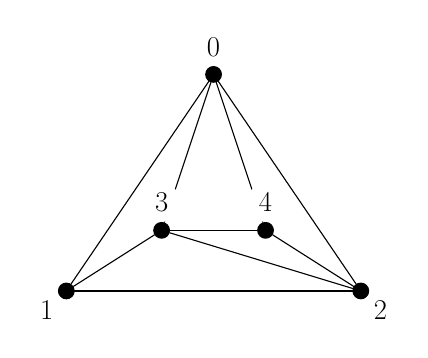
\begin{tikzpicture}
  \node (v0) [label=above:$0$] at (0cm, 2.5cm) {};
  \node (v1) [label=below left:$1$] at (-1.7cm, 0cm) {};
  \node (v2) [label=below right:$2$] at (1.7cm, 0cm) {};
  \node (v3) [label=above:$3$] at (-0.6cm, 0.7cm) {};
  \node (v4) [label=above:$4$] at (0.6cm, 0.7cm) {};
  
  \begin{pgfonlayer}{bg}
	  \draw (v0) edge (v1); \draw (v0) edge (v2); \draw (v2) edge (v1);
	  \draw (v0) edge (v3); \draw (v1) edge (v3); \draw (v0) edge (v4);
	  \draw (v2) edge (v4); \draw (v3) edge (v4); \draw (v2) edge (v3);
  \end{pgfonlayer}
  
\end{tikzpicture}
\end{center}
\caption{A drawing of the graph constructed in Figure \ref{example_make_graph}.}
\end{figure}

Code to construct a simple triangulated planar graph may be seen in Figure
\ref{example_make_graph}. A planar embedding for the graph is constructed
in Figure \ref{example_embed_graph}. 
This graph and embedding will be used as an example input in the later sections.

\begin{figure}
\begin{lstlisting}[frame=single]
// Create a data structure to store the embedding
vector<vector<edge_t>> planar_embedding_storage(
        num_vertices(graph)
    );

// Map each vertex to its rotation scheme
iterator_property_map<
        typename vector<vector<edge_t>>::iterator, 
        property_map<graph_t, vertex_index_t>::const_type
    > planar_embedding(
        planar_embedding_storage.begin(),
        get(vertex_index, graph)
    );

// Researve space so push_back is O(1)
for(size_t v = 0; v < num_vertices(graph); ++v) {
    planar_embedding[v].reserve(out_degree(v, graph));
}

// Construct the planar embedding
boyer_myrvold_planarity_test(
        boyer_myrvold_params::graph = graph,
        boyer_myrvold_params::embedding = planar_embedding
    );
\end{lstlisting}
\caption{Example code to construct a planar embedding in the BGL.}
\label{example_embed_graph}
\end{figure}

We will use \texttt{graph\_t} to refer to some definition of
\texttt{boost::adjacency\_list}. We will use \texttt{vertex\_t} and \texttt{edge\_t}
to refer to the vertex and edge types of \texttt{graph\_t} (see the type
definitions in Figure \ref{example_make_graph} for an example).

\subsection{Poh's Algorithm}

Here we describe our implementation of the linear time Poh algorithm
described in (4.3) and (4.4). The
function prototype, type definitions, and template requirements are shown
in Figures \ref{poh_prototype} and Figure \ref{poh_template}, respectively.

\begin{figure}
\begin{lstlisting}[frame=single]
template<
        typename graph_t,
        typename planar_embedding_t,
        typename color_map_t,
        typename vertex_iterator_t,
        typename color_t
    >
void poh_color(
        const graph_t & graph,
        const planar_embedding_t & planar_embedding,
        vertex_iterator_t p_begin, vertex_iterator_t p_end,
        vertex_iterator_t q_begin, vertex_iterator_t q_end,
        color_t c_0, color_t c_1, color_t c_2,
        color_map_t & color_map
    );
\end{lstlisting}
\caption{Publicly visible function prototype for Poh with Path Walking.}
\label{poh_prototype}
\end{figure}

\begin{figure}
\begin{center}
\begin{tabular}{l|l|l}
Type & Concept & Additional Requirements\\
\hline
\texttt{graph\_t} & none & must be \texttt{adjacency\_list}\\
\texttt{color\_t} & \texttt{EqualityComparable}, & none\\
& \texttt{CopyAssignable} & \\
\texttt{embedding\_t} & \texttt{PlanarEmbedding} & none\\
\texttt{vertex\_iterator\_t} & \texttt{InputIterator} & \texttt{value\_type} is \texttt{vertex\_t}\\
\texttt{color\_map\_t} & \texttt{Lvalue{\allowbreak}Property{\allowbreak}Map} & \texttt{value\_type} is \texttt{color\_t}
\end{tabular}
\end{center}
\caption{Template requirements for Poh with Path Walking.}
\label{poh_template}
\end{figure}

We assume the provided graph is simple and weakly triangulated and the given
planar embedding structure represents a valid planar embedding of the graph.
We assume the two ranges of vertices map are paths in the graph
satisfying the requirements of \textit{Poh -- Path Walk} (4.3).
Finally we assume no vertex is already colored any of \texttt{c\_0}, \texttt{c\_1},
or \texttt{c\_2}.

When the algorithm is complete \texttt{color\_map} will be assigned such that
it represents a valid path $3$-coloring of the subgraph bounded by the cycle
formed by the two provided paths, $\text{Int}(C)$. The coloring will
also satisfy the output requirements of (4.4).

The implementation follows algorithms (4.3) and (4.4) with the following
implementation decisions an modifications. We use a property map to track start
and stop points in the cyclic
ordering of neighbors provided by \texttt{planar\_embedding}, similar to the
neighbor range vertex property described in section 5. This allows us to do a
single iteration through the neighbors of a vertex to get an ``orientation",
then remember this orientation for the remainder of the algorithm.

Additionally, we optimize the implementation by combining the steps of (4.3) and
(4.4). Notice
the path that is colored in (4.4) is the same path we will walk through in a
subsequent call to (4.3). We may therefore perform the marking and chord
finding operations of (4.3) as the path is colored in (4.4). This reduces
the number of times we visit a particular edge by a factor of $2$.

A brief code snippet in Figure \ref{example_poh} shows how to apply Poh to the
graph constructed earlier in Figure \ref{example_make_graph}.
Source code, documentation, and complete examples are available online at the
link provided earlier.

\begin{figure}
\begin{lstlisting}[frame=single]
// Create a data structure to store the coloring
vector<int> color_map_storage(num_vertices(graph));
iterator_property_map<
        vector<int>::iterator,
        typename property_map<
                graph_t, vertex_index_t
            >::const_type
    > color_map(
        color_map_storage.begin(), get(vertex_index, graph)
    );

// Construct the paths P and Q for the example graph
vector<vertex_t> path_p = { 0 };
vector<vertex_t> path_q = { 1, 2 };

// Color the graph with Poh
poh_color(
        graph,
        planar_embedding,
        path_p.begin(), path_p.end(),
        path_q.begin(), path_q.end(),
        1, 2, 3,
        color_map
    );
\end{lstlisting}
\caption{Example code to color a graph with Poh.}
\label{example_poh}
\end{figure}

\begin{figure}
\begin{center}
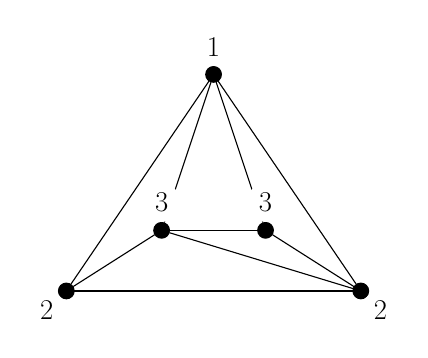
\begin{tikzpicture}
  \node (v0) [label=above:$1$] at (0cm, 2.5cm) {};
  \node (v1) [label=below left:$2$] at (-1.7cm, 0cm) {};
  \node (v2) [label=below right:$2$] at (1.7cm, 0cm) {};
  \node (v3) [label=above:$3$] at (-0.6cm, 0.7cm) {};
  \node (v4) [label=above:$3$] at (0.6cm, 0.7cm) {};
  
  \begin{pgfonlayer}{bg}
	  \draw (v0) edge (v1); \draw (v0) edge (v2); \draw (v2) edge (v1);
	  \draw (v0) edge (v3); \draw (v1) edge (v3); \draw (v0) edge (v4);
	  \draw (v2) edge (v4); \draw (v3) edge (v4); \draw (v2) edge (v3);
  \end{pgfonlayer}
  
\end{tikzpicture}
\end{center}
\caption{The coloring produced by the code in Figure \ref{example_poh}.}
\end{figure}

\subsection{Poh with BFS}

We also provide an implementation of of \textit{Poh -- BFS} (4.2). Note that
the BFS algorithm is slower than the algorithm described in (4.3, 4.4). The
function prototype, type definitions, and template requirements are shown
in Figure \ref{poh_bfs_prototype} and Figure \ref{poh_bfs_template}, respectively.

\begin{figure}
\begin{lstlisting}[frame=single]
template<
        typename graph_t,
        typename planar_embedding_t,
        typename vertex_iterator_t,
        typename color_t,
        typename color_map_t
    >
void poh_color_bfs(
        const graph_t & graph,
        const planar_embedding_t & planar_embedding,
        vertex_iterator_t p_begin, vertex_iterator_t p_end,
        vertex_iterator_t q_begin, vertex_iterator_t q_end,
        color_t c_0, color_t c_1, color_t c_2,
        color_map_t & color_map
    );
\end{lstlisting}
\caption{Publicly visible function prototype for Poh with BFS.}
\label{poh_bfs_prototype}
\end{figure}

\begin{figure}
\begin{center}
\begin{tabular}{l|l|l}
Type & Concept & Additional Requirements\\
\hline
\texttt{graph\_t} & none & must be \texttt{adjacency\_list}\\
\texttt{color\_t} & \texttt{EqualityComparable}, & none\\
& \texttt{CopyAssignable} & \\
\texttt{embedding\_t} & \texttt{PlanarEmbedding} & none\\
\texttt{vertex\_iterator\_t} & \texttt{InputIterator} & \texttt{value\_type} is \texttt{vertex\_t}\\
\texttt{color\_map\_t} & \texttt{Lvalue{\allowbreak}Property{\allowbreak}Map} & \texttt{value\_type} is \texttt{color\_t}
\end{tabular}
\end{center}
\caption{Template requirements for Poh with BFS.}
\label{poh_bfs_template}
\end{figure}

We make the exact same assumptions
about input structures as in our implementation of (4.3, 4.4) in
the previous section.

When the algorithm is complete \texttt{color\_map} will be assigned such that
it represents a valid path $3$-coloring of the subgraph bounded by the cycle
formed by the two provided paths ($\text{Int}(C)$). The coloring will
also satisfy the output requirements of (4.2).

The implementation almost directly follows the description of (4.2), although
some decisions had to be made. In order
to keep the algorithm $\mathcal{O}(n^2)$, we must ensure we iterate through the
adjacency list of a given vertex precisely once during the orientation phase of
(4.2). This is the step where we would locate the position of $v_k$ in
$\text{Adj}[v_1]$. To do this we note that at least one of the path endpoint
vertices $v_1$ or $v_k$ has never been an path endpoint vertex in any call
before. We then always choose this endpoint as the vertex whose adjacency list
we search through.

Source code, documentation, and complete examples are available online at the
link provided earlier.



\subsection{Augmented Embeddings}

In this section we describe the \texttt{Augmented{\allowbreak}Embedding} concept used to store
embedding ordered augmented adjacency lists for a graph.

The \texttt{Augmented{\allowbreak}Embedding} concept refines \texttt{Lvalue{\allowbreak}Property{\allowbreak}Map}, placing
additional restrictions on the \texttt{value\_type} of the map. The types are
described in Figure \ref{augmented_concept}. Valid expressions are described in
Figure \ref{valid_expressions}.

\begin{figure}
\begin{center}
\begin{tabular}{l|l}
Type & \\
\hline
\texttt{augmented\_embedding\_t} &  a type modeling \texttt{Augmented{\allowbreak}Embedding} \\
\texttt{node\_t} & \texttt{boost::property\_traits<augmented\_embedding\_t>}\\
    & $\qquad$\texttt{::value\_type::value\_type}\\
\texttt{iterator\_t} & \texttt{boost::property\_traits<augmented\_embedding\_t>}\\
    & $\qquad$\texttt{::value\_type::iterator}\\
\texttt{graph\_t} & the type of the underlying graph\\
\texttt{vertex\_t} & \texttt{boost::graph\_traits<graph\_t>::vertex\_descriptor}
\end{tabular}
\end{center}
\caption{Types for the AugmentedEmbedding concept.}
\label{augmented_concept}
\end{figure}

The object \texttt{embedding} will assign a range of objects of type
\texttt{node\_t} to each vertex \texttt{v} in the underlying graph. There will be exactly one
node in this range for each neighbor of \texttt{v} in the underlying graph. We will
call this range of nodes the augmented adjacency list for \texttt{v}.

The type \texttt{node\_t} will represent a neighboring vertex \texttt{u} in the augmented
adjacency list for a vertex \texttt{v}. The type \texttt{iterator\_t} will be an iterator for
the range of \texttt{node\_t} objects for a vertex \texttt{v}.

For a vertex \texttt{v} each node \texttt{n} in the range \texttt{embedding{\allowbreak}[v].begin()} to
\texttt{embedding{\allowbreak}[v].end()} will have \texttt{n.vertex} be a neighboring vertex \texttt{u}
and \texttt{n.iterator} be the unique iterator in the range \texttt{embedding{\allowbreak}[u].begin()}
to \texttt{embedding{\allowbreak}[u].end()} such that \texttt{n.iterator{\allowbreak}->vertex} is equal to \texttt{v}.

\begin{figure}
\begin{center}
\begin{tabular}{l|l}
Object(s) & Description\\
\hline
\texttt{u},\texttt{v} & objects of type \texttt{vertex\_t}\\
\texttt{embedding} & an object of type \texttt{augmented\_embedding\_t}\\
\texttt{n} & an object of type \texttt{node\_t}
\end{tabular}
\end{center}
\caption{Notation for our discussion of augmented embeddings.}
\end{figure}
\begin{figure}
\begin{center}
\begin{tabular}{l|l|l}
Expression & Type & Description\\
\hline
\texttt{n.vertex} & \texttt{vertex\_t} & vertex member for the node \texttt{n}\\
\texttt{n.iterator} & \texttt{iterator\_t} & iterator member for the node \texttt{n}\\
\texttt{embedding[v].begin()} & \texttt{iterator\_t} & beginning of the range of nodes\\
\texttt{embedding[v].end()} & \texttt{iterator\_t} & end of the range of nodes\\
\texttt{embedding[v].push\_back(n)} & \texttt{void} & append \texttt{n} to the range of nodes\\
\texttt{embedding[v].clear()} & \texttt{void} & clear the range of nodes
\end{tabular}
\end{center}
\caption{Valid expressions for an object modeling \texttt{Augmented{\allowbreak}Embedding}.}
\label{valid_expressions}
\end{figure}

We implement an algorithm to construct a data structure modeling
\texttt{Augmented{\allowbreak}Embedding}
from a structure modeling \texttt{PlanarEmbedding} based on \textit{Augment
Embedding} (3.1).

A code snippet in Figure \ref{example_augment_embedding} shows how to
construct an augmented embedding structure for the graph from Figure
\ref{example_make_graph}.

\begin{figure}
\begin{lstlisting}[frame=single]
// Struct to store (v,r) pairs for augmented adjacency list
struct adjacency_node_t {
    vertex_t vertex;
    typename vector<adjacency_node_t>::iterator iterator;
};

// Create a structure to store the augmented embedding
vector<vector<adjacency_node_t>> augmented_embedding_storage(
        num_vertices(graph)
    );

// Map each vertex to its augmented adjacency list
iterator_property_map<
        vector<vector<adjacency_node_t>>::iterator,
        typename property_map<
                graph_t, vertex_index_t
            >::const_type
    >  augmented_embedding(
        augmented_embedding_storage.begin(),
        get(vertex_index, graph)
    );

// Researve space so push_back is O(1)
for(size_t v = 0; v < num_vertices(graph); ++v) {
    augmented_embedding[v].reserve(out_degree(v, graph));
}

// Fill in the augmented embedding structure
augment_embedding(
        graph, planar_embedding, augmented_embedding
    );
\end{lstlisting}
\caption{Example code to construct an augmented embedding.}
\label{example_augment_embedding}
\end{figure}

\subsection{Hartman-Skrekovski in the BGL}

Here we detail our implementation of the Hartman-Skrekovski algorithm described
in (5.3, 5.4). The
function prototype and template requirements are shown
in Figure \ref{hartman_prototype} and Figure \ref{hartman_template},
respectively.

\begin{figure}
\begin{lstlisting}[frame=single]
template<
        typename graph_t,
        typename augmented_embedding_t,
        typename color_list_map_t,
        typename face_iterator_t
    >
void hartman_skrekovski_color(
        const graph_t & graph,
        const augmented_embedding_t & augmented_embedding,
        face_iterator_t face_begin, face_iterator_t face_end,
        color_list_map_t & color_list_map
    );
\end{lstlisting}
\caption{Publicly visible function prototype for Hartman-Skrekovski.}
\label{hartman_prototype}
\end{figure}

\begin{figure}
\begin{center}
\begin{tabular}{l|l|l}
Type & Concept & Additional Requirements\\
\hline
\texttt{graph\_t} & none & must be \texttt{adjacency\_list}\\
\texttt{color\_t} & \texttt{EqualityComparable}, & none\\
& \texttt{CopyAssignable} & \\
\texttt{embedding\_t} & \texttt{PlanarEmbedding} & none\\
\texttt{vertex\_iterator\_t} & \texttt{InputIterator} & \texttt{value\_type} is \texttt{vertex\_t}\\
\texttt{color\_list\_t} & \texttt{Sequence{\allowbreak}Container} & \texttt{value\_type} is \texttt{color\_t}\\
\texttt{color\_list\_map\_t} & \texttt{Lvalue{\allowbreak}Property{\allowbreak}Map} & \texttt{value\_type} is \texttt{color\_list\_t}
\end{tabular}
\end{center}
\caption{Template requirements for Hartman-Skrekovski.}
\label{hartman_template}
\end{figure}

We assume the provided graph is simple and weakly triangulated and the given
\texttt{augmented\_embedding} structure represents a valid planar embedding of
the graph.
We assume the range of vertices is a cycle in
the provided plane graph, with vertices listed in clockwise order.
We finally assume \texttt{color\_list\_map} assigns each vertex in the cycle a sequence
of at $2$ or more colors, and each vertex interior to the cycle a sequence of
$3$ or more colors.

When the algorithm is complete \texttt{color\_list\_map} will have been modified
such that a single color remains in each list. The remaining colors will
represent a valid path coloring of the subgraph bounded by the provided cycle
($\text{Int}(C)$).

The implementation follows algorithms (5.3) and (5.4) with the following
optimization. By combining the cases of (5.3) and (5.4) we may draw and remove
the path simultaneously, one vertex at a time. In the implementation therefore
perform the operations of both (5.3) and (5.4) simultaneously as each vertex
is colored. This reduces the number of times we visit a particular edge by a
factor of $2$.

A brief code snippet in Figure \ref{example_hartman} shows how to apply
Hartman-Skrekovski to the graph constructed earlier in Figure \ref{example_make_graph}.
Source code, documentation, and complete examples are available online at the
link provided earlier.

\begin{figure}
\begin{lstlisting}[frame=single]
// Structure listing vertices on the outer cycle
vector<vertex_t> cycle = { 0, 1, 2 };

// Create a structure to store the list assignment
vector<list<int>> color_list_storage(num_vertices(graph));
iterator_property_map<
        vector<list<int>>::iterator,
        typename property_map<
                graph_t, vertex_index_t
            >::const_type
    > color_list_map(
        color_list_storage.begin(), get(vertex_index, graph)
    );

// Assign each vertex a list of the appropriate size
color_list_map[0] = { 1, 2 };
color_list_map[1] = { 2, 3 };
color_list_map[2] = { 1, 4 };
color_list_map[3] = { 1, 3, 4 };
color_list_map[4] = { 1, 2, 4 };

// Construct the path list-coloring
hartman_skrekovski_color(
        graph, augmented_embedding,
        cycle.begin(), cycle.end(),
        color_list_map
    );
\end{lstlisting}
\caption{Example code to color a graph with Hartman-Skrekovski.}
\label{example_hartman}
\end{figure}

\begin{figure}
\begin{center}
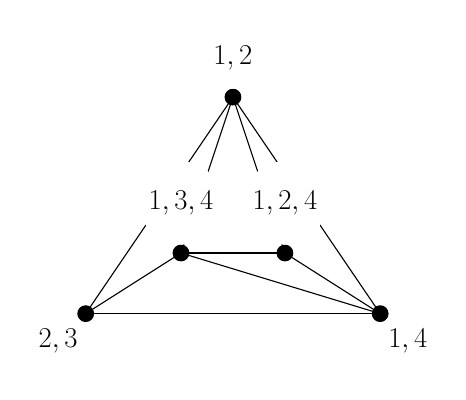
\begin{tikzpicture}
  \node (v0) [label=above:{$1,2$}] at (0cm, 2.5cm) {};
  \node (v1) [label=below left:{$2,3$}] at (-1.7cm, 0cm) {};
  \node (v2) [label=below right:{$1,4$}] at (1.7cm, 0cm) {};
  \node (v3) [label=above:{$1,3,4$}] at (-0.6cm, 0.7cm) {};
  \node (v4) [label=above:{$1,2,4$}] at (0.6cm, 0.7cm) {};
  
  \begin{pgfonlayer}{bg}
	  \draw (v0) edge (v1); \draw (v0) edge (v2); \draw (v2) edge (v1);
	  \draw (v0) edge (v3); \draw (v1) edge (v3); \draw (v0) edge (v4);
	  \draw (v2) edge (v4); \draw (v3) edge (v4); \draw (v2) edge (v3);
  \end{pgfonlayer}
  
\end{tikzpicture}
$\qquad$
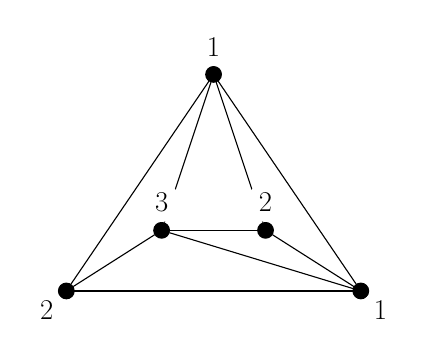
\begin{tikzpicture}
  \node (v0) [label=above:$1$] at (0cm, 2.5cm) {};
  \node (v1) [label=below left:$2$] at (-1.7cm, 0cm) {};
  \node (v2) [label=below right:$1$] at (1.7cm, 0cm) {};
  \node (v3) [label=above:$3$] at (-0.6cm, 0.7cm) {};
  \node (v4) [label=above:$2$] at (0.6cm, 0.7cm) {};
  
  \begin{pgfonlayer}{bg}
	  \draw (v0) edge (v1); \draw (v0) edge (v2); \draw (v2) edge (v1);
	  \draw (v0) edge (v3); \draw (v1) edge (v3); \draw (v0) edge (v4);
	  \draw (v2) edge (v4); \draw (v3) edge (v4); \draw (v2) edge (v3);
  \end{pgfonlayer}
  
\end{tikzpicture}
\end{center}
\caption{The coloring produced by the code in Figure \ref{example_hartman}.}
\end{figure}

\section{Conclusion}

In this project we considered two inductive procedures on plane graphs: one
computing a path $3$-colorings, and one computing a path list-coloring with
lists of size at least $3$. We adapted each procedure to an
algorithm for finding path colorings of graphs with adjacency list
representations. Additionally, we showed each procedure admits an algorithm that
runs in linear time.
Finally, we implemented each algorithm in C++ and give instructions for
using each algorithm, alongside example code.

Future work in this area might consider Hartman's procedure for path
$4$-coloring torus graphs, also found in \cite{hartman}. The procedure first
cuts and collapses a noncontractible cycle in the torus graph to form a plane
graph. It then divides the resulting plane graph
into several subgraphs which are individually colored with Poh's algorithm.
The combined coloring may then be adapted to a path $4$-coloring of the original
torus graph. It would be interesting to see if this procedure might be adapted to
a linear time algorithm.

\begin{comment}

\begin{figure}
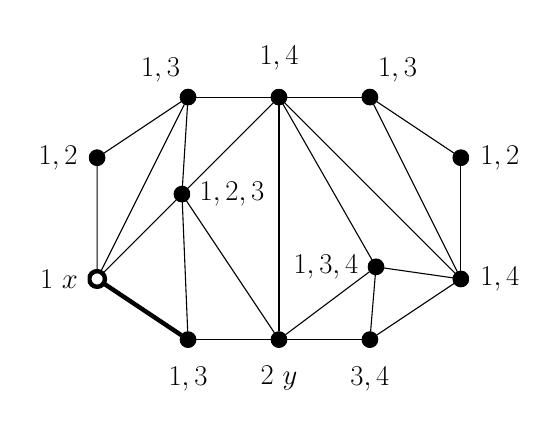
\begin{tikzpicture}[scale=0.7]
	\node (1) [label=left:{$1,2$}] at (-3.0cm, 1.0cm) {};
	\node (2) [label=above left:{$1,3$}] at (-1.5cm, 2.0cm) {};
	\node (3) [label=above:{$1,4$}] at (0.0cm, 2.0cm) {};
	\node (4) [label=above right:{$1,3$}] at (1.5cm, 2.0cm) {};
	\node (5) [label=right:{$1,2$}] at (3.0cm, 1.0cm) {};
	\node (6) [label=right:{$1,4$}] at (3.0cm, -1.0cm) {};
	\node (7) [label=below:{$3,4$}] at (1.5cm, -2.0cm) {};
	\node (8) [label=below:{$2 \ y$}] at (0.0cm, -2.0cm) {};
	\node (9) [label=below:{$1,3$}] at (-1.5cm, -2.0cm) {};
	\node (10) [label=left:{$1 \ x$}, ultra thick, fill=white] at (-3.0cm, -1.0cm) {};
	\node (11) [label=right:{$1,2,3$}] at (-1.6cm, 0.4cm) {};
	\node (12) [label=left:{$1,3,4$}] at (1.6cm, -0.8cm) {};
	
	\draw (1) edge (2); \draw (2) edge (3); \draw (3) edge (4);
	\draw (4) edge (5); \draw (5) edge (6); \draw (6) edge (7);
	\draw (7) edge (8); \draw (8) edge (9); \draw (9) edge (10) [ultra thick];
	\draw (10) edge (1);
	
	\draw (2) edge (11); \draw (3) edge (11); \draw (3) edge (6);
	\draw (4) edge (6); \draw (3) edge (8); \draw (7) edge (12);
	\draw (8) edge (11); \draw (9) edge (11); \draw (10) edge (11);
	\draw (10) edge (2); \draw (3) edge (12); \draw (6) edge (12);
	\draw (8) edge (12);
\end{tikzpicture}
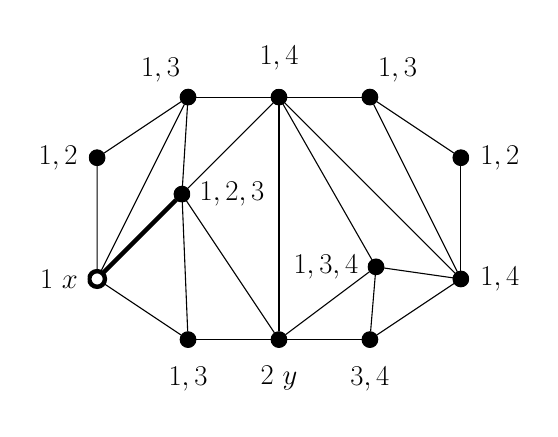
\begin{tikzpicture}[scale=0.7]
	\node (1) [label=left:{$1,2$}] at (-3.0cm, 1.0cm) {};
	\node (2) [label=above left:{$1,3$}] at (-1.5cm, 2.0cm) {};
	\node (3) [label=above:{$1,4$}] at (0.0cm, 2.0cm) {};
	\node (4) [label=above right:{$1,3$}] at (1.5cm, 2.0cm) {};
	\node (5) [label=right:{$1,2$}] at (3.0cm, 1.0cm) {};
	\node (6) [label=right:{$1,4$}] at (3.0cm, -1.0cm) {};
	\node (7) [label=below:{$3,4$}] at (1.5cm, -2.0cm) {};
	\node (8) [label=below:{$2 \ y$}] at (0.0cm, -2.0cm) {};
	\node (9) [label=below:{$1,3$}] at (-1.5cm, -2.0cm) {};
	\node (10) [label=left:{$1 \ x$}, ultra thick, fill=white] at (-3.0cm, -1.0cm) {};
	\node (11) [label=right:{$1,2,3$}] at (-1.6cm, 0.4cm) {};
	\node (12) [label=left:{$1,3,4$}] at (1.6cm, -0.8cm) {};
	
	\draw (1) edge (2); \draw (2) edge (3); \draw (3) edge (4);
	\draw (4) edge (5); \draw (5) edge (6); \draw (6) edge (7);
	\draw (7) edge (8); \draw (8) edge (9); \draw (9) edge (10);
	\draw (10) edge (1);
	
	\draw (2) edge (11); \draw (3) edge (11); \draw (3) edge (6);
	\draw (4) edge (6); \draw (3) edge (8); \draw (7) edge (12);
	\draw (8) edge (11); \draw (9) edge (11); \draw (10) edge (11) [ultra thick];
	\draw (10) edge (2); \draw (3) edge (12); \draw (6) edge (12);
	\draw (8) edge (12);
\end{tikzpicture}
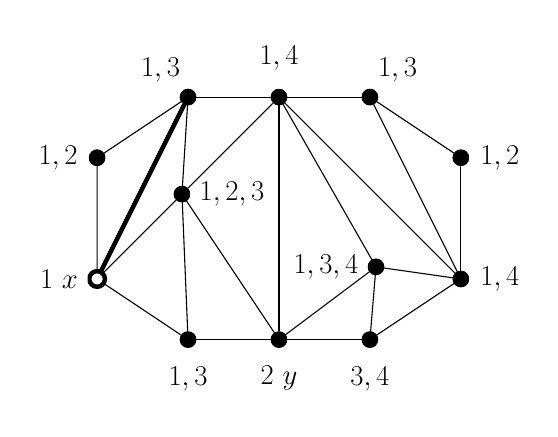
\begin{tikzpicture}[scale=0.7]
	\node (1) [label=left:{$1,2$}] at (-3.0cm, 1.0cm) {};
	\node (2) [label=above left:{$1,3$}] at (-1.5cm, 2.0cm) {};
	\node (3) [label=above:{$1,4$}] at (0.0cm, 2.0cm) {};
	\node (4) [label=above right:{$1,3$}] at (1.5cm, 2.0cm) {};
	\node (5) [label=right:{$1,2$}] at (3.0cm, 1.0cm) {};
	\node (6) [label=right:{$1,4$}] at (3.0cm, -1.0cm) {};
	\node (7) [label=below:{$3,4$}] at (1.5cm, -2.0cm) {};
	\node (8) [label=below:{$2 \ y$}] at (0.0cm, -2.0cm) {};
	\node (9) [label=below:{$1,3$}] at (-1.5cm, -2.0cm) {};
	\node (10) [label=left:{$1 \ x$}, ultra thick, fill=white] at (-3.0cm, -1.0cm) {};
	\node (11) [label=right:{$1,2,3$}] at (-1.6cm, 0.4cm) {};
	\node (12) [label=left:{$1,3,4$}] at (1.6cm, -0.8cm) {};
	
	\draw (1) edge (2); \draw (2) edge (3); \draw (3) edge (4);
	\draw (4) edge (5); \draw (5) edge (6); \draw (6) edge (7);
	\draw (7) edge (8); \draw (8) edge (9); \draw (9) edge (10);
	\draw (10) edge (1);
	
	\draw (2) edge (11); \draw (3) edge (11); \draw (3) edge (6);
	\draw (4) edge (6); \draw (3) edge (8); \draw (7) edge (12);
	\draw (8) edge (11); \draw (9) edge (11); \draw (10) edge (11);
	\draw (10) edge (2) [ultra thick]; \draw (3) edge (12); \draw (6) edge (12);
	\draw (8) edge (12);
\end{tikzpicture}
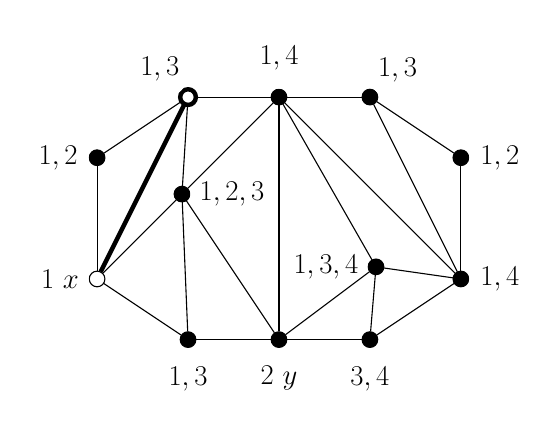
\begin{tikzpicture}[scale=0.7]
	\node (1) [label=left:{$1,2$}] at (-3.0cm, 1.0cm) {};
	\node (2) [label=above left:{$1,3$}, ultra thick, fill=white] at (-1.5cm, 2.0cm) {};
	\node (3) [label=above:{$1,4$}] at (0.0cm, 2.0cm) {};
	\node (4) [label=above right:{$1,3$}] at (1.5cm, 2.0cm) {};
	\node (5) [label=right:{$1,2$}] at (3.0cm, 1.0cm) {};
	\node (6) [label=right:{$1,4$}] at (3.0cm, -1.0cm) {};
	\node (7) [label=below:{$3,4$}] at (1.5cm, -2.0cm) {};
	\node (8) [label=below:{$2 \ y$}] at (0.0cm, -2.0cm) {};
	\node (9) [label=below:{$1,3$}] at (-1.5cm, -2.0cm) {};
	\node (10) [label=left:{$1 \ x$}, fill=white] at (-3.0cm, -1.0cm) {};
	\node (11) [label=right:{$1,2,3$}] at (-1.6cm, 0.4cm) {};
	\node (12) [label=left:{$1,3,4$}] at (1.6cm, -0.8cm) {};
	
	\draw (1) edge (2); \draw (2) edge (3); \draw (3) edge (4);
	\draw (4) edge (5); \draw (5) edge (6); \draw (6) edge (7);
	\draw (7) edge (8); \draw (8) edge (9); \draw (9) edge (10);
	\draw (10) edge (1);
	
	\draw (2) edge (11); \draw (3) edge (11); \draw (3) edge (6);
	\draw (4) edge (6); \draw (3) edge (8); \draw (7) edge (12);
	\draw (8) edge (11); \draw (9) edge (11); \draw (10) edge (11);
	\draw (10) edge (2) [ultra thick]; \draw (3) edge (12); \draw (6) edge (12);
	\draw (8) edge (12);
\end{tikzpicture}
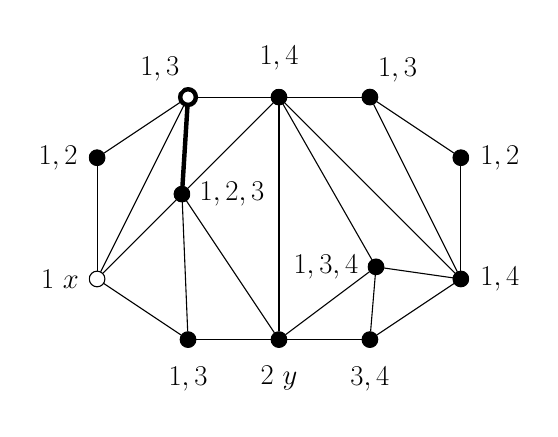
\begin{tikzpicture}[scale=0.7]
	\node (1) [label=left:{$1,2$}] at (-3.0cm, 1.0cm) {};
	\node (2) [label=above left:{$1,3$}, ultra thick, fill=white] at (-1.5cm, 2.0cm) {};
	\node (3) [label=above:{$1,4$}] at (0.0cm, 2.0cm) {};
	\node (4) [label=above right:{$1,3$}] at (1.5cm, 2.0cm) {};
	\node (5) [label=right:{$1,2$}] at (3.0cm, 1.0cm) {};
	\node (6) [label=right:{$1,4$}] at (3.0cm, -1.0cm) {};
	\node (7) [label=below:{$3,4$}] at (1.5cm, -2.0cm) {};
	\node (8) [label=below:{$2 \ y$}] at (0.0cm, -2.0cm) {};
	\node (9) [label=below:{$1,3$}] at (-1.5cm, -2.0cm) {};
	\node (10) [label=left:{$1 \ x$}, fill=white] at (-3.0cm, -1.0cm) {};
	\node (11) [label=right:{$1,2,3$}] at (-1.6cm, 0.4cm) {};
	\node (12) [label=left:{$1,3,4$}] at (1.6cm, -0.8cm) {};
	
	\draw (1) edge (2); \draw (2) edge (3); \draw (3) edge (4);
	\draw (4) edge (5); \draw (5) edge (6); \draw (6) edge (7);
	\draw (7) edge (8); \draw (8) edge (9); \draw (9) edge (10);
	\draw (10) edge (1);
	
	\draw (2) edge (11) [ultra thick]; \draw (3) edge (11); \draw (3) edge (6);
	\draw (4) edge (6); \draw (3) edge (8); \draw (7) edge (12);
	\draw (8) edge (11); \draw (9) edge (11); \draw (10) edge (11);
	\draw (10) edge (2); \draw (3) edge (12); \draw (6) edge (12);
	\draw (8) edge (12);
\end{tikzpicture}
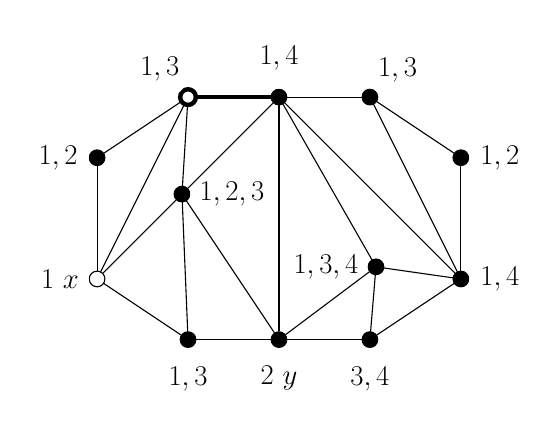
\begin{tikzpicture}[scale=0.7]
	\node (1) [label=left:{$1,2$}] at (-3.0cm, 1.0cm) {};
	\node (2) [label=above left:{$1,3$}, ultra thick, fill=white] at (-1.5cm, 2.0cm) {};
	\node (3) [label=above:{$1,4$}] at (0.0cm, 2.0cm) {};
	\node (4) [label=above right:{$1,3$}] at (1.5cm, 2.0cm) {};
	\node (5) [label=right:{$1,2$}] at (3.0cm, 1.0cm) {};
	\node (6) [label=right:{$1,4$}] at (3.0cm, -1.0cm) {};
	\node (7) [label=below:{$3,4$}] at (1.5cm, -2.0cm) {};
	\node (8) [label=below:{$2 \ y$}] at (0.0cm, -2.0cm) {};
	\node (9) [label=below:{$1,3$}] at (-1.5cm, -2.0cm) {};
	\node (10) [label=left:{$1 \ x$}, fill=white] at (-3.0cm, -1.0cm) {};
	\node (11) [label=right:{$1,2,3$}] at (-1.6cm, 0.4cm) {};
	\node (12) [label=left:{$1,3,4$}] at (1.6cm, -0.8cm) {};
	
	\draw (1) edge (2); \draw (2) edge (3) [ultra thick]; \draw (3) edge (4);
	\draw (4) edge (5); \draw (5) edge (6); \draw (6) edge (7);
	\draw (7) edge (8); \draw (8) edge (9); \draw (9) edge (10);
	\draw (10) edge (1);
	
	\draw (2) edge (11); \draw (3) edge (11); \draw (3) edge (6);
	\draw (4) edge (6); \draw (3) edge (8); \draw (7) edge (12);
	\draw (8) edge (11); \draw (9) edge (11); \draw (10) edge (11);
	\draw (10) edge (2); \draw (3) edge (12); \draw (6) edge (12);
	\draw (8) edge (12);
\end{tikzpicture}
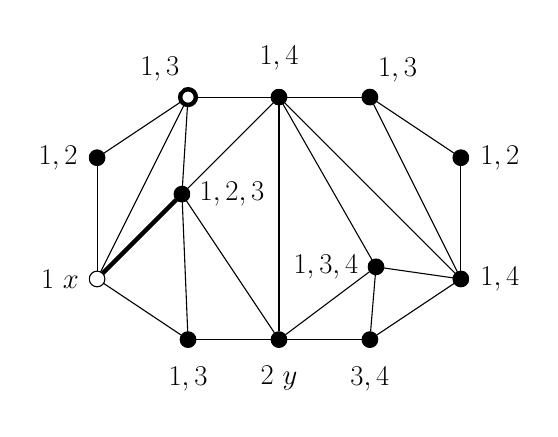
\begin{tikzpicture}[scale=0.7]
	\node (1) [label=left:{$1,2$}] at (-3.0cm, 1.0cm) {};
	\node (2) [label=above left:{$1,3$}, ultra thick, fill=white] at (-1.5cm, 2.0cm) {};
	\node (3) [label=above:{$1,4$}] at (0.0cm, 2.0cm) {};
	\node (4) [label=above right:{$1,3$}] at (1.5cm, 2.0cm) {};
	\node (5) [label=right:{$1,2$}] at (3.0cm, 1.0cm) {};
	\node (6) [label=right:{$1,4$}] at (3.0cm, -1.0cm) {};
	\node (7) [label=below:{$3,4$}] at (1.5cm, -2.0cm) {};
	\node (8) [label=below:{$2 \ y$}] at (0.0cm, -2.0cm) {};
	\node (9) [label=below:{$1,3$}] at (-1.5cm, -2.0cm) {};
	\node (10) [label=left:{$1 \ x$}, fill=white] at (-3.0cm, -1.0cm) {};
	\node (11) [label=right:{$1,2,3$}] at (-1.6cm, 0.4cm) {};
	\node (12) [label=left:{$1,3,4$}] at (1.6cm, -0.8cm) {};
	
	\draw (1) edge (2); \draw (2) edge (3); \draw (3) edge (4);
	\draw (4) edge (5); \draw (5) edge (6); \draw (6) edge (7);
	\draw (7) edge (8); \draw (8) edge (9); \draw (9) edge (10);
	\draw (10) edge (1);
	
	\draw (2) edge (11); \draw (3) edge (11); \draw (3) edge (6);
	\draw (4) edge (6); \draw (3) edge (8); \draw (7) edge (12);
	\draw (8) edge (11); \draw (9) edge (11); \draw (10) edge (11)  [ultra thick];
	\draw (10) edge (2); \draw (3) edge (12); \draw (6) edge (12);
	\draw (8) edge (12);
\end{tikzpicture}
\end{figure}

\end{comment}

%\section{Boost Graph Implementation}




\begin{thebibliography}{99}
\bibitem{jacobson}
	Andrews, J. A. and Michael S. Jacobson, On a generalization of chromatic number,
	\textit{Congressus Numerantium} \textbf{47} (1985), 33-48.
\bibitem{appel1}
	Appel, K. and W. Haken, Every planar map is four colorable. I.
	Discharging, \textit{Illinois J. Math} \textbf{21} (1991), no. 3, 429-490.
\bibitem{appel2}
	Appel, K. and W. Haken, Every planar map is four colorable. II.
	Reducibility, \textit{Illinois J. Math} \textbf{21} (1991), no. 3, 491-567.
\bibitem{booth}
	Booth, K. and C. Lueker, Testing for the consecutive ones property interval
	graphs and graph planarity using $PQ$-tree algorithms," \textit{J. Comput.
	System Sci.} \textbf{13} (1976), 335-379.
\bibitem{boyer}
	Boyer, J. and W. Myrvold, On the cutting edge: simplified $\mathcal{O}(n)$ planarity by
	edge addition, \textit{J. Graph Algorithms Appl.} \textbf{8} (2004), 241-273.
\bibitem{broere}
	Broere, I. and C. M. Mynhardt, Generalized colorings of outerplanar and planar
	graphs, \textit{Graph theory with applications to algorithms and computer
	science (Kalamazoo, Mich., 1984)}, 151-161, Wiley-Intersci. Publ., Wiley,
	New York, 1985.
\bibitem{chappell}
    Bross, A., G. G. Chappell, and C. Hartman, Path
    coloring algorithms for plane graphs, in preparation.
\bibitem{chartrand}
	Chartrand, G., D. P. Geller, and S. Hedetniemi, A generalization of the
	chromatic number, \textit{Proc. Cambridge Philos. Soc.} \textbf{64} (1968),
	265-271.
\bibitem{kronk}
    Chartrand, G. and H. V. Kronk, The point-arboricity of planar graphs,
    \textit{J. London. Math. Soc.} \textbf{44} (1969), 612-616.
\bibitem{cowen}
	Cowen, L., R. Cowen, and D. Woodall, Defective colorings of graphs in
	surfaces: partitions into subgraphs of bounded valency,
	\textit{J. Graph Theory} \textbf{10} (1986), 187-195.
\bibitem{hull}
	Eaton, N. and N. Hull, Defective list colorings of planar graphs,
	\emph{Bull. Inst. Combin. Appl.} \textbf{25} (1999), 79-87.
\bibitem{erdos}
	Erd{\"o}s, P., A. Rubin, H. Taylor, Choosability in graphs,
	\textit{Congressus Numerantium} \textbf{26} (1980), 125-157.
\bibitem{eswaran}
	Eswaran, K. and R. Tarjan, Augmentation problems, \textit{SIAM J. Comput.}
	\textbf{5} (1976), 653-665.
\bibitem{goddard}
    Goddard, W., Acyclic colorings of planar graphs, \textit{Discrete Math}
    \textbf{91} (1991), 91-94.
\bibitem{hagerup}
	Hagerup, T. and C. Uhrig, Triangulating a planar graph, \textit{Library of
	Efficient Datatypes and Algorithms}, software package, Max Planck Institute
	for Informatics, Saarbr{\"u}cken, 1991.
\bibitem{jones}
	Harary, F. and K. Jones, Conditional colorability II: bipartite variations,
	Proceedings of the Sundance conference on combinatorics and related topics
	(Sundance, Utah, 1985), \textit{Congressus Numerantium} \textbf{50} (1985),
	205-218.
\bibitem{hartman}
	Hartman, C. M.,
	\textit{Extremal Problems in Graph Theory}, Ph.D. Thesis, University of Illinois,
	1997.
\bibitem{tarjan}
	Hopcroft, J. and E. Tarjan, Efficient planarity testing, \textit{J. Assoc.
	Comput. Mach.} \textbf{21} (1974), 549-568.
\bibitem{lempel}
	Lempel, A., S. Even, and I. Cederbaum, An algorithm for planarity testing of
	graphs, \textit{Theory of graphs (Internat. Sympos., Rme, 1966)}, 215-232,
	Gordon and Breach, New York; Dunod, Paris.
\bibitem{poh}
	Poh, K. S., On the linear vertex-arboricity of a planar graph,
	\emph{J. Graph Theory} \textbf{14} (1990), 73-75.
\bibitem{reed}
	Reed, R., A new method for drawing a planar graph given the cyclic order of the
	edges at each vertex, Sixteenth Manitoba conference on numerical
	mathematics and computing (Winnipeg, Man., 1986), \textit{Congressus
	Numerantium} \textbf{56} (1987), 31-44.
\bibitem{boost}
	Siek, J., L. Lee, and A. Lumsdaine, \textit{The Boost Graph Library: User
	Guide and Reference Manual}, Pearson Education, 2001.
\bibitem{skrekovski}
	Skrekovski, R., List improper colourings of planar graphs,
	\textit{Combin. Probab. Comput.} \textbf{8} (1999), 293-299.
\bibitem{thomassen}
	Thomassen, C., Every planar graph is $5$-choosable,
	\emph{J. Combin. Theory Ser. B} \textbf{62} (1994), no. 1, 180-181.
\bibitem{voigt}
	Voigt, M., List colorings of planar graphs,
	\textit{Discrete Mathematics} \textbf{120}, 215-219.
\bibitem{west}
	West, D., \textit{Introduction to Graph Theory},
	2nd ed., Pearson, 2001.
\end{thebibliography}

\begin{comment}
\appendix
\section{Code}
\subsection{Poh with breadth first search (4.2)}
%\inputminted{C++}{../../src/path_coloring/poh_color_bfs.hpp}

\subsection{Poh with face tracing (4.3, 4.4)}
%\inputminted{C++}{../../src/path_coloring/poh_color.hpp}

\subsection{Hartman-Skrekovski (5.3, 5.4)}
%\inputminted{C++}{../../src/path_coloring/hartman_skrekovski_choose.hpp}

\subsection{Embedding helper functions}

\subsection{Disjoint set structure}

\end{comment}

\end{document}
